
% Inspirado en:
%   https://es.overleaf.com/latex/templates/tesis-universidad-de-murcia-umu-eidum/pspmjbxvpfff
% Notas: 
%   - "estilos": variables.tex donde poner titulo, autor, etc... y otros de librerías etc...
%   - "capitulos": capitulos
%   - "capitulos/tablas": tablas
%   - "img": imagenes

\documentclass[a4paper,12pt,oneside]{book}
% phd-estilo-basico.tex
% aml! 2015-09-08. amaurandi@um.es
% ------------------------------------------------

%\documentclass[a4paper,12pt]{book}
%\documentclass[11pt]{book}
%\usepackage[paperwidth=17cm, paperheight=22.5cm, bottom=2.5cm, right=2.5cm]{geometry}
\usepackage{amssymb,amsmath,amsthm} %paquete para símbolo matemáticos
%\usepackage{apacite} %para usar APA cite en bibligrafia tb modificar
% \usepackage[spanish, es-nodecimaldot]{babel}  % ponemos tabla en vez de cuadro, sep decimal el punto (Us- notation)
\usepackage[spanish, es-tabla, es-nodecimaldot]{babel}  % ponemos tabla en vez de cuadro, sep decimal el punto (Us- notation)

%\usepackage{ucs}
\usepackage[utf8x]{inputenc} %Paquete para escribir acentos y otros símbolos directamente

\usepackage{pdflscape}
\usepackage{multirow, booktabs,setspace,caption,longtable}
\usepackage{tikz}

% Cambios FV:
% \DeclareCaptionLabelSeparator*{spaced}{\\[2ex]}
% \captionsetup[table]{textfont=it,format=plain,justification=justified,
%   singlelinecheck=false,labelsep=spaced,skip=0pt}
% \captionsetup[figure]{labelsep=period,labelfont=it,justification=justified,
%   singlelinecheck=false,font=doublespacing}

\usepackage[figuresleft]{rotating}
% \usepackage{enumerate}
\usepackage{enumitem}
\usepackage{graphicx}
\usepackage[nottoc]{tocbibind}


\setlength{\parskip}{3mm}

%\usepackage[pdftex,
%            pdfauthor={Your Name},
%            pdftitle={The Title},
%            pdfsubject={The Subject},
%            pdfkeywords={Some Keywords},
%            pdfproducer={Latex with hyperref, or other system},
%            pdfcreator={pdflatex, or other tool}]{hyperref}

\usepackage[
	%paperwidth=17cm,     % como hago para que trome A4 (sin meterle los cms)???
	%paperheight=23.5cm, 
	inner=1.5cm,
	outer=1.5cm,
	top=2.5cm,
	bottom=2cm,
	bindingoffset=1cm]{geometry}

\setlength{\captionmargin}{20pt}

%\usepackage[table, xcdraw]{xcolor}

% % bloques verbarin coloreados segun estilo Rstudio para código R
% % ------------------------------------------------
% \usepackage{color}
% \usepackage{fancyvrb}
% \newcommand{\VerbBar}{|}
% \newcommand{\VERB}{\Verb[commandchars=\\\{\}]}
% \DefineVerbatimEnvironment{Highlighting}{Verbatim}{commandchars=\\\{\}}
% % Add ',fontsize=\small' for more characters per line
% \usepackage{framed}
% \definecolor{shadecolor}{RGB}{248,248,248}
% \newenvironment{Shaded}{\begin{snugshade}}{\end{snugshade}}
% \newcommand{\KeywordTok}[1]{\textcolor[rgb]{0.13,0.29,0.53}{\textbf{{#1}}}}
% \newcommand{\DataTypeTok}[1]{\textcolor[rgb]{0.13,0.29,0.53}{{#1}}}
% \newcommand{\DecValTok}[1]{\textcolor[rgb]{0.00,0.00,0.81}{{#1}}}
% \newcommand{\BaseNTok}[1]{\textcolor[rgb]{0.00,0.00,0.81}{{#1}}}
% \newcommand{\FloatTok}[1]{\textcolor[rgb]{0.00,0.00,0.81}{{#1}}}
% \newcommand{\CharTok}[1]{\textcolor[rgb]{0.31,0.60,0.02}{{#1}}}
% \newcommand{\StringTok}[1]{\textcolor[rgb]{0.31,0.60,0.02}{{#1}}}
% \newcommand{\CommentTok}[1]{\textcolor[rgb]{0.56,0.35,0.01}{\textit{{#1}}}}
% \newcommand{\OtherTok}[1]{\textcolor[rgb]{0.56,0.35,0.01}{{#1}}}
% \newcommand{\AlertTok}[1]{\textcolor[rgb]{0.94,0.16,0.16}{{#1}}}
% \newcommand{\FunctionTok}[1]{\textcolor[rgb]{0.00,0.00,0.00}{{#1}}}
% \newcommand{\RegionMarkerTok}[1]{{#1}}
% \newcommand{\ErrorTok}[1]{\textbf{{#1}}}
% \newcommand{\NormalTok}[1]{{#1}}
% % ------------------------------------------------

\usepackage{pdfpages} % insertar pdf en los anexos
%\usepackage{cite} % para contraer referencias

\usepackage{fancyhdr}
\pagestyle{fancy}

\usepackage{placeins}  % para usar \FloatBarrier
%\usepackage{minitoc}
\usepackage{float}

\usepackage{lipsum}
\usepackage{setspace}

\usepackage{caption}

% BIBLIOGRAFIA (FV):
% \usepackage{biblatex}
% \usepackage[style=apa]{biblatex}
% \addbibresource{ref.bib}

% \usepackage{bibentry}
% \bibliographystyle{apalike}
%\bibliographystyle{unsrt} % igual q plain pero numera en orden de aparición
%\bibliographystyle{apacite}
%\bibliographystyle{plainnat}
% \usepackage{apacite} %para usar APA cite en bibligrafia tb modificar \bibliographystyle{apacite} en su ssitio 
% \DefineBibliographyStrings{spanish}{ andothers = {et\addabbrvspace al\adddot}, and = {y}, }
% \renewcommand{\BOthers}[1]{et al.\hbox{}}
% \addto\captionsspanish{
	%   \renewcommand{\BOthers}[1]{et al.\hbox{}}
	% }
	
%aml para solventar el tema de las citas intex.. 20220405
\usepackage[sort&compress,square,comma,authoryear]{natbib}
% FV para poder incluir full cite con \bibentry:
\usepackage{bibentry}

\usepackage{url}
\usepackage{hyperref}

\nobibliography*


% makes color citations
%\usepackage[colorlinks=true,urlcolor=blue,citecolor=red,linkcolor=red,bookmarks=true]{hyperref}


% \usepackage{ulem} %para tachar frases
 

\usepackage{titlesec}
\definecolor{gray75}{gray}{0.75}
\newcommand{\hsp}{\hspace{4pt}}

\titlespacing*{\chapter}{0pt}{0pt}{20pt}

\titleformat{\chapter}[display]
    {\normalfont\huge\bfseries\raggedright}
    {\chaptertitlename\ \thechapter}{10pt}{\LARGE}
% \titlespacing*{\chapter}{0pt}{0pt}{20pt}
% \chaptertitlefont{\fontsize{22pt}{30pt}\selectfont}

% \titleformat{\chapter}[display]
%   {\bfseries\small\raggedleft}
%   {\normalfont\huge\bfseries}{\chaptertitlename\ \thechapter}
%   {10pt}
%   {\LARGE}
  
  % {\raggedright\bfseries\small}
  % {\small\chaptertitlename \resizebox{!}{0.2cm}{\,\thechapter\,}}

\titleformat{\section}[hang]
  {\Large\bfseries}
  {\thesection\hsp\hsp}
  {0pt}
  {\Large\bfseries}

\titleformat{\subsection}[hang]
  {\large\bfseries}
  {\thesubsection.\hsp\hsp}
  {0pt}
  {\large\bfseries}


% FV comandos/operadores nuevos:
% \newcommand{\biaspmi}{\text{Bias}_{\operatorname{PMI}}}
\DeclareMathOperator{\PMI}{PMI}
\DeclareMathOperator{\BiasPMI}{Bias_{PMI}}
\DeclareMathOperator{\BiasWE}{Bias_{WE}}

% \newcommand{\variableTituloTesis}{Este Es el Título}
% \newcommand{\variableTesinando}{Francisco Tomás Valentini}
% \newcommand{\variableAnho}{2023}
% \newcommand{\variableDireccionUno}{Dr. Edgar Altszyler}


\begin{document}

\frontmatter % start roman page numbering

% PORTADA
\pagestyle{empty} % No page number here

\begin{titlepage}


    % \vspace{28.5mm}

    \begin{figure}[!htb]
        \centering
        
\includegraphics[width=5cm]{img/institucional/1200px-Logo-fcenuba.png}
    \end{figure}


    \begin{center}
        \Large{\textbf{UNIVERSIDAD DE BUENOS AIRES}}
        \vspace{3mm}
        \\ \normalsize{FACULTAD DE CIENCIAS EXACTAS Y NATURALES}
        \vspace{6mm}
    \end{center}


    \vspace{8mm}
    \begin{center}
        \LARGE{\textbf{Estimación de sesgos en textos con Pointwise Mutual Information (PMI)}}
        \vspace{13mm}
        % la frase siguiente textual
        \\ \normalsize{Tesis Presentada para Optar al Título de Magíster en Explotación de Datos y Descubrimiento del Conocimiento}
        \vspace{13mm}
    \end{center}

    \vspace{20mm}

    \begin{minipage}[t]{0.9\textwidth}
        {\normalsize{\textbf{Tesista: }}{\normalsize{Lic. Francisco Tomás Valentini}}}\\ \\
        % \vspace{5mm}   \\
        {\normalsize{\textbf{Director: }}{\normalsize{Dr. Edgar Altszyler}}}\\ \\
        %  \vspace{5mm}   
        {\normalsize{\textbf{Co-Director: }}{\normalsize{Dr. Germán Rosati}}}\\ \\
        % \vspace{5mm}
        %si corresponde
        {\normalsize{\textbf{Lugar de trabajo: }}{\normalsize{Laboratorio de Inteligencia Artificial Aplicada (LIAA) en el Instituto de Ciencias de la Computación (ICC)}}}\\ \\
        % \vspace{5mm}
        {\normalsize{\textbf{Buenos Aires, }}{\normalsize{1° de abril de 2025}}}
    \end{minipage}

    % \vspace*{\fill}

\end{titlepage}

% \newpage 
% \ % pagina en blanco
% \newpage

% % CONTRAPORTADA con nombres de directoras
% % portada.tex

\FloatBarrier
\vspace{28.5mm}
%Figura
\begin{figure}[H]
    \begin{center}
        
\includegraphics[width=72mm]{img/institucional/logo-uba.png}
    \end{center}
\end{figure}


\begin{center}



%\vspace{7.5mm}
\textsc{\Large UNIVERSIDAD DE BUENOS AIRES}\\[4em]

%\vspace{28mm}
\textsc{\Large Maestría en Explotación de Datos y Descubrimiento del Conocimiento}\\[4em]


\vspace{20mm}
\textsc{\Large \variableTituloTesis    } 



\vspace{20mm}
\textsc{\Large \variableTesinando}\\[1em]
\textsc{\Large \variableAnho}\\[1em]

\large Dirección: \\ \variableDireccionUno
% \large Dirección: \\ \variableDireccionUno \\ \variableDireccionDos \\ \variableDireccionTres


\end{center}

\vspace*{\fill}


%\end{titlepage}





%\newpage

% % AGRADECIMIENTOS
% \chapter*{Agradecimientos}
% %\markboth{AGRADECIMIENTOS23}{AGRADECIMIENTOS} % encabezado 
% %agradecimientos.tex

\lipsum[1-4]


% PREFACIO

\chapter*{Prefacio}

Esta tesis de maestría está basada en los hallazgos presentados en la siguiente publicación, la cual es el resultado de las investigaciones realizadas durante el desarrollo de la tesis:

\bibentry{valentini2023problems}


%En este trabajo emplearemos las siguientes convenciones: 

%\begin{itemize}
%\item 
%Se empleará la tipografía \textit{cursiva} para palabras en otro idioma distinto del castellano y para resaltar nombres como, por ejemplo, los nombres de variables.
%\item 
%Emplearemos la tipografía \texttt{código} para sentencias de código,  nombres de funciones y librerías de \texttt{R}.
%\item 
%Emplearemos el punto como separador decimal, por ejemplo: \texttt{1/2=0.5}, y un espacio simple como separador de millares, por ejemplo: \texttt{123\;345} tal como recomienda la Academia de la Lengua Española en la Ortografía del 2010, página 666 \cite{espanola2010ortografia}. 
%\item 
%Cuando informemos sobre una media, la acompañaremos entre paréntesis de la desviación típica, por ejemplo: \texttt{8.81(1.21)}. 
%\item 
%Si informamos de un porcentaje, entre paréntesis, incluimos la frecuencia absoluta, por ejemplo: \texttt{50.25\%(123)}, o viceversa: \texttt{123(50.25\%)}. 
%\item 
%En las tablas de descriptivos, empleamos la abreviatura \texttt{SD} para \emph{desviación estandar} (del inglés \emph{Standard  Deviation}).
%\item 
%En el texto empleamos la abreviatura \texttt{EPV} para \emph{Enfermedades Prevenibles por Vacunas}.
%\end{itemize}



% RESUMEN

\chapter*{Resumen}

En los últimos años se ha extendido el uso de los \emph{word embeddings} para medir sesgos y estereotipos sociales en textos. Las métricas basadas en \emph{word embeddings} han demostrado su eficacia en la detección de una amplia variedad de sesgos pero carecen de transparencia e interpretabilidad. En esta tesis introducimos y analizamos una métrica alternativa basada en \emph{Pointwise Mutual Information} (PMI) para medir sesgos en textos. Mostramos que esta métrica, a diferencia de las métricas basadas en \emph{word embeddings}: (1) puede expresarse como una función de probabilidades condicionales, lo que proporciona una interpretación sencilla en términos de coocurrencias de palabras, y (2) permite estimar intervalos de confianza y la significación estadística de los resultados paramétricamente. Realizamos un conjunto de experimentos para comparar la métrica basada en PMI con las métricas basadas en \emph{word embeddings} en tres dimensiones: estimación de la variabilidad, correlación con el juicio humano e interpretabilidad. Los resultados sirven para ilustrar las ventajas del método basado en PMI, así como también la diferencia fundamental en el tipo de asocaciones semánticas que capturan. El código usado para realizar esta tesis está disponible en \url{https://github.com/ftvalentini/tesis-SesgoPMI}.

% A partir de un conjunto de experimentos, mostramos que, además de las ventajas en términos de interpretabilidad y fiabilidad de la inferencia estadística, el enfoque basado en PMI produce resultados similares a los de las métricas basadas en \emph{embeddings} a la hora de captar las diferencias de género del mundo real incrustadas en grandes corpus.


%-------------------------------------------------------------------
% TABLA DE CONTENIDOS
%-------------------------------------------------------------------

%\setcounter{tocdepth}{1}
%level -1: part, 0: chapter, 1: section, etc.
\renewcommand{\baselinestretch}{0.1}\normalsize
\tableofcontents
\renewcommand{\baselinestretch}{0.3}\normalsize
\listoffigures
\renewcommand{\baselinestretch}{0.3}\normalsize
\listoftables
\renewcommand{\baselinestretch}{1.2}\normalsize


%-------------------------------------------------------------------
%	TESIS
%-------------------------------------------------------------------

\mainmatter % start arabic page numbering
\pagestyle{headings}

% \def\tablename{Tabla}% para que denomine tabla a las tablas y no "cuadro"
%\doublespacing
\onehalfspace
%\singlespace
%\spacing{1.5}	
\setlength{\parskip}{3mm} % separación entre párrafo
\setlength{\parindent}{1cm} % indentación primera linea de párrafo


\chapter{Introducción} \label{cap:intro}

% Estructura:
% - motivacion
% - sesgos en modelos vs sesgos en textos
% - objetivos / preguntas
% - organizacion


El campo de investigación de la equidad en la Inteligencia Artificial (\emph{fairness in AI}) ha recibido una gran atención en los últimos años, impulsado por la necesidad de que los algoritmos basados en aprendizaje automático tomen decisiones imparciales y no discriminatorias. Los sesgos en los sistemas de Inteligencia Artificial emergen por la \textbf{replicación y amplificación de los sesgos presentes en los datos de entrenamiento}. Por consiguiente, es fundamental estudiar exhaustivamente estos sesgos y desarrollar métodos computacionales dentro del dominio del Procesamiento del Lenguaje Natural (NLP) que puedan medir eficaz y confiablemente los sesgos de los textos usados para entrenar estos algoritmos. 

Además, la medición de sesgos mediante técnicas computacionales es de gran importancia en las \textbf{ciencias sociales computacionales} porque permite analizar cómo se representan los distintos grupos sociales en productos culturales como libros, películas, revistas, diarios y redes sociales. Un estudio riguroso de los métodos de cuantificación de sesgos en textos es fundamental para entender la reproducción de estereotipos relacionados con el género, la nacionalidad y otras características.

La medición de los sesgos en los textos, entendida como \textbf{una tarea diferente a la medición de los sesgos de los modelos de aprendizaje automático}, tiene su propia importancia. Mientras que una parte importante de las investigaciones anteriores se han centrado predominantemente en medir los sesgos de los modelos (\citealp{bolukbasi2016man,kiritchenko2018examining,zhao2018gender,bordia2019identifying,gonen2019lipstick,lu2020gender,blodgett2020language}, por mencionar algunos ejemplos ampliamente citados), es esencial comprender y cuantificar los sesgos inherentes a los propios textos. Esta tesis pretende proporcionar una herramienta analítica fiable para abordar esta tarea, la cual es especialmente valiosa para los estudios de ciencias sociales computacionales. 

En este campo, \textbf{se ha vuelto extendido el uso de \emph{word embeddings} para medir sesgos y estereotipos sociales en \emph{corpora}}. Los \emph{embeddings}, representaciones de palabras como vectores densos, capturan asociaciones semánticas entre palabras basadas en sus patrones de coocurrencia en el \emph{corpus}. Aunque han demostrado ser útiles para detectar una amplia variedad de sesgos, las métricas basadas en \emph{embeddings} carecen de transparencia e interpretabilidad. Cuando se usan \emph{embeddings} para medir sesgos, es difícil determinar si los resultados se deben a asociaciones de primer orden generalizadas o si se derivan de asociaciones de orden superior poco claras. Esta falta de interpretabilidad dificulta la comprensión de los aspectos específicos del \emph{corpus} que contribuyen a las mediciones de sesgo. Además, las métricas existentes basadas en \emph{embeddings} no proporcionan un medio eficiente y confiable de estimar los intervalos de confianza o la significación estadística.

% que suelen realizarse utilizando incrustaciones estáticas de palabras. Pretendemos ir más allá de las métricas basadas en la incrustación de palabras, que carecen de transparencia, interpretabilidad y explicabilidad. Nuestra métrica alternativa, basada en la información mutua puntual (PMI), ofrece una interpretación sencilla en términos de coocurrencias de palabras y permite estimar intervalos de confianza y significación estadística.

Para abordar estas limitaciones, \textbf{presentamos una métrica alternativa basada en \emph{Pointwise Mutual Information} (PMI) para medir sesgos en textos}. PMI es una medida de asociación de primer orden entre dos palabras que compara sus probabilidades de ocurrencia individuales con su probabilidad de coocurrencia. La métrica basada en PMI tiene una interpretación transparente y ofrece la posibilidad de estimar intervalos de confianza y evaluar la significación estadística de manera confiable. Esto permite a los investigadores comprender mejor las relaciones semánticas específicas que dan lugar a las estimaciones de sesgo, así como también obtener conclusiones más sólidas acerca de la presencia y la magnitud de los sesgos en los textos.

Los \textbf{objetivos de esta tesis} son dos. En primer lugar, buscamos analizar la métrica basada en PMI para medir sesgos en textos, estudiando sus propiedades estadísticas y sus ventajas de interpretabilidad, que hasta ahora se habían pasado por alto. En segundo lugar, nos proponemos evaluar las diferencias, ventajas y desventajas del método basado en PMI frente a las técnicas existentes basadas en \emph{embeddings}. Para ello, realizamos un conjunto de experimentos en la Wikipedia en inglés que apuntan a comparar ambas métricas en tres dimensiones: estimación de la variabilidad, correlación con el juicio humano e interpretabilidad. 


La organización de esta tesis es la siguiente. El \textbf{capítulo \ref{cap:sesgo_textos}} hace una revisión de la literatura sobre la medición de sesgos en textos con herramientas de NLP, enfocándose predominantemente en las métricas basadas en \emph{word embeddings}. Describimos los métodos más difundidos para entrenar \emph{embeddings} y las métricas típicamente usadas para medir sesgos con éstos. El \textbf{capítulo \ref{cap:bias_pmi}} presenta los fundamentos teóricos de la métrica de medición de sesgos basada en PMI, explicando su interpretación en términos de coocurrencias. También presenta la estimación de los intervalos de confianza y la significación estadística dentro de este marco. En el \textbf{capítulo \ref{cap:experimentos}} realizamos experimentos orientados a ilustrar las propiedades de la métrica basada en PMI en términos de estimación de la variabilidad, correlación con el juicio humano e interpretabilidad. Describimos la configuración experimental, los conjuntos de datos usados, y las metodologías de evaluación empleadas, y luego presentamos los resultados. Finalmente, el \textbf{capítulo \ref{cap:conclusiones}} concluye la tesis, resumiendo las contribuciones y discutiendo las implicaciones de nuestros hallazgos.
 
El código utilizado en esta tesis está disponible en \url{https://github.com/ftvalentini/tesis-SesgoPMI} para su uso y exploración.

% ----------------------------------------------------------------------------




\chapter{Medición de sesgos textuales} \label{cap:sesgo_textos}

A los fines de este trabajo, definimos el \textbf{sesgo textual} como el grado en que el lenguaje usado para describir grupos o cosas es diferente \citep{hoyle2019unsupervised}. Algunos de estos sesgos pueden ser moralmente neutrales, como por ejemplo, el sesgo según el cual los insectos son relativamente desagradables, mientras que las flores son agradables. En cambio, los sesgos derivados de aspectos de la cultura humana que pueden conducir a comportamientos dañinos, como los sesgos de género o de nacionalidad, pueden ser problemáticos y llevan el nombre de sesgos estereotipados o directamente \textbf{estereotipos} \citep{caliskan2017semantics}. 

Típicamente, la literatura sobre sesgos en el NLP se centra en el estudio de estereotipos porque su reproducción es potencialmente perjudicial para la sociedad. La metodología más usada para medir sesgos textuales son las métricas basadas en \emph{word embeddings} estáticos, los cuales describimos a continuación.


\section{\emph{Word embeddings} estáticos} \label{sec:embeddings}

% [qué son los WE estáticos]
Los \emph{embeddings} son \textbf{representaciones vectoriales densas} de las palabras de un corpus que tienen dimensión relativamente baja (usualmente entre 50 y 1000 dimensiones). Los \emph{embeddings} que usamos en este trabajo y que se usan típicamente para medir sesgos textuales son estáticos. Esto significa que cada palabra del vocabulario se representa con un \textbf{único vector fijo}, diferenciándose de las representaciones contextualizadas que se desarrollaron posteriormente, donde las palabras tienen \emph{embeddings} distintos según el contexto en el que se encuentran (por ejemplo, los \emph{embeddings} BERT de \citealp{devlin2019bert}). 

Los espacios vectoriales de los \emph{embeddings} estáticos se generan a partir de la distribución de las palabras en el \emph{corpus}, bajo la hipótesis de que las palabras que aparecen en contextos similares suelen tener un contenido semántico similar. Con esta metodología, el significado de las palabras intenta aprenderse a partir de sus \textbf{coocurrencias}, es decir, de la frecuencia de palabras que aparecen en su contexto cercano. Durante el proceso de aprendizaje de los vectores, se busca que los vectores de palabras semánticamente asociadas estén relativamente cerca en el espacio vectorial, y los de palabras no asociadas, relativamente lejos. 

A continuación describimos los tres métodos de generación de \emph{word embeddings} que usamos en este trabajo.

\subsection{\emph{Skip-gram with negative sampling} (SGNS)} \label{sec:sgns}

%[qué es SGNS]
La metodología de \emph{Skip-gram with negative sampling} (SGNS) \citep{mikolov2013distributed} representa a cada palabra del vocabulario con dos vectores de igual dimensión: un \textbf{vector objetivo $v_w$} y un \textbf{vector de contexto $v_c$}. Los parámetros que se buscan aprender son entonces dos matrices, $W$ y $C$, cada una de las cuales contiene en cada fila el \emph{embedding} o vector de cada una de las palabras del vocabulario. 

Estos parámetros se ajustan para optimizar una función de pérdida donde los pares de palabras que efectivamente coocurren en el corpus se toman como ejemplos positivos, mientras que como ejemplos negativos se toman muestras aleatorias del vocabulario, llamadas \textbf{muestras negativas}.

Más específicamente, los ejemplos positivos son los pares de palabras $(w,c)$ que surgen de considerar una ventana de tamaño $2\,T$ alrededor de cada palabra $w$, donde $w$ es la palabra central, $T$ es el tamaño de la ventana, y las palabras en la ventana son las palabras de contexto $c$. Por cada ejemplo positivo $(w,c)$ se muestrean $k$ palabras usando la distribución de probabilidad de de ocurrencia de cada palabra estimada con  
%
\begin{equation}
    P_{\alpha}(i) = \frac{f(i)^{\alpha}}{\sum_{j \in V} f(j)^{\alpha}}
\end{equation}
%
donde $f(i)$ es la cantidad de veces que una palabra $i$ coocurre con cualquier otra palabra en el corpus, $V$ es el vocabulario y $\alpha$ es un parámetro de suavizado. Estos $k$ ejemplos son los ejemplos negativos o \emph{palabras de ruido}. El parámetro $0 < \alpha < 1$ suaviza la distribución, incrementando la probabilidad de muestrear palabras con baja frecuencia porque $P_{\alpha}(i) > P(i)$ para palabras relativamente poco frecuentes. 

% NOTE esto impacta directamente en el v_c de low freq words --> no es obvio que genere mejores representaciones de v_w para low freq words // la motivacion de que es util es un rdo mas bien empirico?

Para entrenar los parámetros $W$ y $C$, para cada ejemplo positivo $(w,c)$ junto con sus $k$ ejemplos negativos se minimiza una \textbf{función de pérdida} definida como: 

\begin{equation}
    L(w,c) = -\log \sigma(v_c^T v_w) - \sum_{i=1}^k \log \sigma(-v_{n_i}^T v_w)
\end{equation}

$\sigma$ es la función sigmoidea, de modo que $\sigma(v_c^T v_w)$ modela la probabilidad de que la palabra $c$ sea una palabra de contexto real para la palabra objetivo $w$, mientras que la probabilidad de que una palabra $c$ no sea una palabra de contexto real para $w$ se modela como $\sigma(-v_{c}^T v_w)$. Entonces, la función de pérdida $L$ arroja valores bajos cuando la probabilidad asignada a que $c$ sea una palabra de contexto real para $w$ es alta, y cuando las probabilidades asignadas a que los ejemplos negativos $n_i$ sean palabras de contexto reales para $w$ son bajas.

Esta función de pérdida se minimiza con \textbf{descenso por el gradiente} tomando como parámetros ajustables los vectores $v_w$ y $v_c$, almacenados en las matrices $W$ y $C$. Más específicamente, se usan los ejemplos positivos y negativos como datos de entrenamiento, se inicializan aleatoriamente $W$ y $C$, y se recorren los datos de entrenamiento aplicando descenso por el gradiente, ajustando los pesos de $W$ y $C$ de manera tal que la similitud $\sigma(v_c^T v_w)$ de los pares $(w, c)$ que efectivamente ocurren en el corpus tienda a maximizarse, a la vez que se minimice la similitud de los pares que no ocurren en el corpus (ejemplos negativos). 

Como resultado, una vez alcanzado un número máximo de pasadas por el \emph{corpus}, las palabras que tienden a coocurrir en las ventanas de coocurrencia tienden a tener representaciones cercanas en el espacio vectorial, mientras que las palabras que aparecen en contextos diferentes tienden a representarse con vectores que están relativamente lejos.

En las librerías más populares que implementan SGNS (como \texttt{gensim} de \citealp{rehurek2010gensim}, que usamos en este trabajo), se tiende a usar únicamente el vector $v_w$ como representación vectorial final de cada palabra, mientras que el vector $v_c$ se descarta.


\subsection{FastText} \label{sec:fasttext}

%[qué es FastText]
Los \emph{embeddings} generados con SGNS sólo están definidos para palabras que son parte de $V$, el vocabulario de entrenamiento. Es decir, no es posible obtener \emph{embeddings} para palabras que no estén en el \emph{corpus} de entrenamiento (\textbf{palabras OOV}, \emph{out-of-vocabulary}) pero que puedan ser de interés, como las distintas formas o inflexiones asociadas a verbos y sustantivos.

Para resolver esto, la metodología FastText \citep{bojanowski2017enriching} representa a cada palabra como sí misma más el conjunto de n-gramas o \textbf{subpalabras} que la constituyen. Para ello, se añaden símbolos especiales \texttt{<} y \texttt{>} al comienzo y final de la palabra antes de hacer la partición en subpalabras. Luego se aprenden vectores para cada subpalabra con la misma metodología de entrenamiento que SGNS. En general se consideran como subpalabras todos los n-gramas de entre 3 y 6 caracteres que componen a la palabra.

Finalmente, para obtener el vector final de palabras OOV se calcula el promedio de los vectores de las subpalabras que la constituyen que existen en el vocabulario, mientras que para palabras que sí están en $V$ se incluye también en el promedio el vector de la palabra completa. Por ejemplo, si la palabra \emph{gato} está en el vocabulario, su vector final será el promedio de los vectores 
de los 3-gramas \texttt{<ga}, \texttt{gat}, \texttt{ato}, \texttt{to>}, los 4-gramas \texttt{<gat}, \texttt{gato}, \texttt{ato>}, y los 5-gramas \texttt{<gato}, \texttt{gato>}, y el vector de la palabra completa \texttt{<gato>}. En el presente trabajo consideramos únicamente palabras que están en $V$.

Al igual que en SGNS, se suelen considerar únicamente los vectores $v_w$, mientras que los vectores $v_c$ se descartan. 

\subsection{GloVe} \label{sec:glove}

% [qué es GloVe]
En lugar de recorrer todos los pares de coocurrencias a la hora de aprender los \emph{embeddings}, la metodología GloVe (\emph{Global Vectors for Word Representation}, \citealp{pennington2014glove}) busca aprovechar los conteos globales almacenados en la \textbf{matriz de coocurrencias $M$}, la cual se precalcula antes de iniciar el entrenamiento. La misma almacena en cada celda $M_{ij}$ la cantidad de veces que la palabra $i$ aparece en el contexto de la palabra $j$ en el \emph{corpus} de entrenamiento al considerar una ventana de tamaño $2\,T$ alrededor de cada palabra.

La función de pérdida GloVe para el \emph{corpus} en su conjunto viene dada por 
%
\begin{equation} \label{eq:glove_loss}
    L = \sum_{i,j=1}^V f(M_{ij}) (v_{w_i}^T v_{c_j} + v_{b_w} + v_{b_c} - \log M_{ij})^2
\end{equation}
%
donde $M_{ij}$ indica el número de veces que la palabra $j$ aparece en el contexto de la palabra $i$, $v_{w_i}$ es el vector objetivo de la palabra $i$, $v_{c_j}$ es el vector de contexto de la palabra $j$, y $v_{b_w}$ y $v_{b_c}$ son son escalares específicos para cada palabra que funcionan como interceptos. $f(M_{ij})$ es una función de ponderación de las coocurrencias que se define como
%
\begin{equation}
    f(x) = \begin{cases}
        \left(\frac{x}{x_{\text{max}}}\right)^\alpha & \text{si } x < x_{\text{max}} \\
        1 & \text{si } x \geq x_{\text{max}}
    \end{cases}
\end{equation}
%
Con esta función se reduce el peso de las coocurrencias poco frecuentes (porque $f(x) < 1$ para $x < x_{\text{max}}$). \citet{pennington2014glove} usan $\alpha = 0.75$, lo cual incrementa ligeramente el peso de las coocurrencias más pequeñas (porque $f(x)_{\alpha=0.75} > f(x)_{\alpha=1}$ para $x < x_{\text{max}}$), de manera similar a como lo hace el parámetro de \emph{smoothing} $\alpha$ de SGNS. En este trabajo mantenemos este valor.
% , a la vez que se evita que las coocurrencias más frecuentes dominen la función de pérdida (porque $f(x)=1$ para $x > x_{\text{max}}$).
%donde $x_{\text{max}}$ es el máximo conteo de coocurrencias que se considera, y $\alpha$ es un parámetro que controla la ponderación de los conteos de coocurrencias. \citet{pennington2014glove} usan los valores de $x_{\text{max}} = 100$ y $\alpha = 0.75$, los cuales mantenemos en este trabajo. 

La pérdida de la ecuación \ref{eq:glove_loss} se minimiza cuando $v_{w_i}^T v_{c_j} + v_{b_w} + v_{b_c} = \log M_{ij}$. Para optimizar la función se muestrean aleatoria e iterativamente tandas de elementos no nulos de la matriz $M$ para calcular los gradientes de los parámetros $v_{w_i}$, $v_{c_j}$, $v_{b_w}$ y $v_{b_c}$, y luego actualizarlos con el algoritmo AdaGrad \citep{duchi2011adaptive}. El entrenamiento finaliza cuando se alcanza un número máximo de pasadas completas por la matriz de coocurrencias.

Al igual que SGNS y FastText, el modelo genera dos conjuntos de vectores de palabras, $W$ y $C$. Dado que $M$ es simétrica, $W$ y $C$ son conceptualmente equivalentes y sólo difieren por tener inicializaciones aleatorias distintas. Por lo tanto, por defecto, los \emph{embeddings} GloVe de una palabra $i$ se obtienen sumando los vectores objetivo y de contexto de la misma ($v_{w_i} + v_{c_i}$). 


\section{Medición de sesgos con \emph{word embeddings}} \label{sec:bias_we}

%[cómo medir sesgos con WE]
Dado que miden la similitud semántica entre las palabras de un corpus, los \emph{word embeddings} son ampliamente utilizados para \textbf{cuantificar sesgos textuales de \emph{corpora} específicos}. La metodología consiste en entrenar \emph{embeddings} sobre el \emph{corpus} que se desea estudiar, y luego computar una \textbf{métrica de medición de sesgo textual}.

En la versión más general, se conforman dos conjuntos de \textbf{palabras de contexto $A$ y $B$}, y un conjunto de \textbf{palabras objetivo $X$}. El sesgo textual de las palabras $X$ en relación a los atributos $A$ y $B$ en un \emph{corpus} dado se mide calculando la diferencia de similitudes entre $X$ con respecto a $A$ y $B$:

\begin{equation} \label{eq:bias}
    \text{Bias}(X,A,B) = \text{sim}(X,A) - \text{sim}(X,B)
\end{equation}

Las medidas de sesgo textual cuantifican, entonces, cuánto más se asocian las palabras de $X$ con las de $A$ que con las de $B$. La similitud semántica se puede cuantificar con la \textbf{similitud coseno} entre \emph{word embeddings} (WE), de manera que el sesgo para una palabra objetivo individual $x$ queda definida como:
%
\begin{equation} \label{eq:bias_we}
    \BiasWE(x,A,B) =
    \frac{1}{|A|} \sum_{a \in A} \text{cos}(v_x,v_a) -
    \frac{1}{|B|} \sum_{b \in B} \text{cos}(v_x,v_b)
\end{equation}
%
donde $v_i$ es el vector de la palabra $i$ y $\text{cos}(v_i,v_j)$ es la similitud coseno entre vectores \citep{lewis2020gender}.

Por ejemplo, siguiendo a \citet{lewis2020gender}, para medir el $\BiasWE$ de género binario (femenino vs masculino) en un \emph{corpus} en inglés, los conjuntos $A$ y $B$ se pueden conformar con palabras que representan a los géneros femenino y masculino, respectivamente: $A$ = \{$female$, $woman$, $she$,...\} y $B$ = \{$male$, $man$, $he$,...\}. Las palabras $x$, por su parte, son aquellas donde es de interés medir estereotipos, por ejemplo, ocupaciones como \emph{nurse}, \emph{doctor}, \emph{engineer}, etc. En el caso en que se desea medir el sesgo conjuntamente para un conjunto de palabras $X$, se toma el promedio de $\BiasWE$ a lo largo de las $x$ que conforman el conjunto. 

%[antecedentes medicion de sesgo con WE]
En la literatura que estudia sesgos lingüísticos, múltiples estudios han usado variantes de la ecuación \ref{eq:bias_we} para \textbf{analizar corpus específicos}. Por ejemplo, \citet{garg2018word} entrenaron \emph{embeddings} GloVe en el \emph{New York Times Annotated Corpus} para cuantificar los cambios en los estereotipos hacia las mujeres y las minorías étnicas en los Estados Unidos a lo largo del siglo XX. Para este análisis, usaron métricas basadas en la distancia euclidiana y la similitud coseno muy similares a la ecuación \ref{eq:bias_we}, y explicaron que ambas arrojaban resultados similares.

\citet{kozlowski2019geometry}, por otro lado, entrenaron embeddings SGNS en libros digitalizados disponibles en Google Ngrams para examinar la evolución de los sesgos de etnia, género y clase a lo largo del tiempo. La métrica que utilizaron primero calcula la diferencia promedio entre los vectores de $N$ palabras de contexto apareadas (es decir, $d = \frac{1}{N} \sum_{i=1}^N v_{a_i}-v_{b_i}$), y luego toma la similitud coseno de esta dirección con el vector de la palabra objetivo, $v_x$ i.e. $\text{cos}(d,v_x)$.

% es decir, $\frac{1}{N} \sum_{i=1}^N \text{cos}(v_{a_i},v_{b_i})$

% NOTE Bolukbasi toma 10 pares ai-bi, calcula los 10 PCs, y se queda con el 1er PC como la dirección de genero ("g") -- luego hacer cos(x, g)

\citet{lewis2020gender} midieron sesgos de género con la ecuación \ref{eq:bias_we} usando \emph{embeddings} FastText entrenados en Wikipedias y subtítulos de 25 idiomas. Descubrieron que los sesgos de género medidos en pruebas de asociaciones psicológicas implícitas están estrechamente relacionados con los sesgos de género textuales de la lengua que hablan los participantes de las pruebas.

Otro estudio, el de \citet{charlesworth2021gender}, midió los estereotipos de género relacionados con las ocupaciones y los rasgos de personalidad con \emph{embeddings} FastText en \emph{corpora} de diversos dominios (por ejemplo, conversaciones de niños y adultos, libros, películas, televisión). Encontraron que los sesgos eran estables a pesar de las diferencias en los \emph{corpora}.

Otro tipo de estudios han usado \textbf{\emph{embeddings} pre-entrenados sobre grandes volúmenes de texto, en lugar de entrenar desde cero} \emph{embeddings} sobre \emph{corpora} de interés. Esto les ha permitido estudiar los sesgos que podrían existir potencialmente en el \emph{corpus} de entrenamiento. 

Uno de los trabajos más destacados de este tipo es el de \citet{caliskan2017semantics}, quienes midieron los sesgos de género en vectores GloVe pre-entrenados en el \emph{corpus} Common Crawl, obtenido de un barrido de la web a gran escala \citep{pennington2014glove}. Encontraron una correlación entre los sesgos de género de los \emph{embeddings} y la distribución del género en los nombres de personas y en las ocupaciones en Estados Unidos. Para realizar este análisis, utilizaron la métrica SC-WEAT (\emph{Single-Category Word Embedding Association Test}, \citealp{toney2021valnorm}), que agrega el desvío estándar de las similitudes de $v_x$ con respecto al conjunto de vectores de $A \cup B$ como denominador de la ecuación \ref{eq:bias_we}. Esta misma medida también se usó en el estudio de \citet{charlesworth2021gender}.

%Caliskan et al. (2017). They use pretrained embeddings as “a tool to extract associations captured in text corpora” and find that “text corpora contain recoverable and accurate imprints of our historic biases”. 

En otro estudio relevante, \citet{garg2018word} analizaron las tendencias de los estereotipos a lo largo de la historia utilizando los \emph{embeddings} HistWords pre-entrenados con \emph{Google Books} y el \emph{Corpus of Historical American English} \citep{hamilton2016diachronic}. De manera similar, \citet{jones2020stereotypical} utilizaron los HistWords para analizar la trayectoria en el tiempo de las asociaciones estereotipadas de género en la lengua inglesa escrita desde el 1800 hasta el 2000. Para medir los sesgos, usaron una métrica parecida a la ecuación \ref{eq:bias_we}, pero adaptada a múltiples palabras objetivo: la similitud entre $X$ y las palabras de contexto, por ejemplo $\text{sim}(X,A)$, se computa tomando el promedio de las similitudes de todas las combinaciones posibles de pares $(x_i,a_i)$, donde $x_i \in X$ y $a_i \in A$.

Por otro lado, \citet{defranza2020language} usaron \emph{embeddings} FastText pre-entrenados en las Wikipedias y Common Crawls de 45 idiomas distintos para analizar los pensamientos voluntarios de las personas expresados en los textos de cada idioma. La métrica que usaron para medir sesgos textuales es similar a la de la ecuación \ref{eq:bias_we}, pero adaptada al caso en que se cuenta con dos grupos de palabras objetivo. Esto es útil en los idiomas en los que las palabras tienen género gramatical. Sus resultados mostraron que los sesgos textuales de género son más frecuentes en las lenguas con género gramatical que en las que no lo tienen.

% TODO Lenton et al., 2009 TODO contar?; 
% TODO Kulkarni et al., 2015 TODO contar?; 

En el presente trabajo usamos la especificacion de la ecuación \ref{eq:bias_we} por su flexibilidad: no requiere palabras de contexto apareadas, admite grupos de contexto de distinta longitud y puede calcularse si los grupos de contexto están conformados por una sola palabra cada uno (esto último no es posible en una métrica como el SC-WEAT). Además, no precisamos extenderla para el caso de palabras con género gramatical porque trabajamos con el idioma inglés, en el que las palabras no tienen género gramatical.

\subsection{Estimación de la variabilidad de métricas basadas en \emph{word embeddings}} \label{sec:bias_we_variabilidad}

%[IC / pvalue de sesgos con WE]

Las métricas basadas en \emph{embeddings} admiten el uso de técnicas de remuestreo para estimar la variabilidad del estadístico específico que se esté calculando. Esto permite evaluar la robustez de los resultados obtenidos. 


Por una parte, la literatura ha usado \textbf{tests de permutaciones para calcular la significancia estadística} de $\text{Bias}_{\text{WE}}$ o métricas similares \citep{caliskan2017semantics,charlesworth2021gender}. Los tests de permutaciones consisten en asignar aleatoriamente las palabras de contexto entre entre los grupos $A$ y $B$ en múltiples iteraciones y calcular la métrica de sesgo en cada iteración. Con los valores del sesgo de cada iteración se construye la distribución nula del sesgo, y se calcula el p-valor a dos colas como la fracción de veces que el valor absoluto del sesgo de la distribución nula es igual o mayor que el observado \citep{north2002note}.

Por otro lado, se ha usado \textbf{bootstrap para obtener intervalos de confianza} con un enfoque de remuestreo parecido a los tests de permutaciones \citep{garg2018word}. En este caso, en cada iteración de bootstrap se muestrean las palabras de contexto $A$ y $B$ por separado con reemplazo y se calcula la métrica de sesgo. Con los valores del sesgo de cada iteración se construye la distribución de bootstrap del sesgo. El error estándar del sesgo se estima luego como la desviación estándar de la distribución de bootstrap, y los cuantiles de la distribución se utilizan para obtener intervalos de confianza \citep{davison1997bootstrap}.

Destacamos que, en rigor, los intervalos de confianza computados por \citet{garg2018word} hacen bootstrap sobre las palabras objetivo y estiman entonces la variabilidad del sesgo cuando se computa para muchas palabras objetivo en simultáneo. Sin embargo, este enfoque se puede extender a las palabras de contexto cuando se computa el sesgo de una sola palabra objetivo, como en nuestro caso.

Otro enfoque, propuesto por \citet{kozlowski2019geometry}, consiste en estimar la variabilidad del sesgo que se origina en la variabilidad propia de los \emph{embeddings}. El método consiste en entrenar múltiples conjuntos de \emph{embeddings} sobre subconjuntos del \emph{corpus} (e.g. 20) y estimar el desvío estándar e intervalo de confianza en base a estas realizaciones. Si bien consideramos que este enfoque es válido, no lo implementamos por ser computacionalmente costoso para \emph{corpora} relativamente grandes, como el que usamos en esta tesis.

% TODO borrar esto:?
En resumen, la estimación de la variabilidad de las métricas sesgo textual es fundamental para evaluar la robustez de los resultados obtenidos. Los métodos de remuestreo, como los tests de permutaciones y el bootstrap, son las herramientas típicamente usadas para lograr este objetivo en el caso de métricas basadas en \emph{word embeddings}.


\chapter{Medición de sesgos con PMI} \label{cap:bias_pmi}

% TODO sacar cosas de esta intro que esten en otros lados:
Hemos mostrado que los enfoques basados en \emph{embeddings} estáticos se han usado ampliamente para detectar y cuantificar sesgos en \emph{corpora}. Estos vectores pueden usarse para medir la similitud semántica entre palabras y, por lo tanto, detectar patrones de sesgo en el uso de ciertas palabras. Si bien los \emph{embeddings} son una herramienta poderosa para medir similitud, y por lo tanto, sesgos, no son la única. El \textbf{Pointwise Mutual Information (PMI)} es una medida que también puede usarse para medir la similitud semántica entre palabras. 

A continuación, describiremos la medida de PMI y presentaremos una métrica para cuantificar sesgos textuales basado en esta medida. Como veremos en los capitulos subsiguientes, la introducción de esta métrica se justifica por su mayor transparencia e interpretabilidad.
% TODO agregar lo de variabilidad si queda en este capitulo

\section{Antecedentes} \label{sec:pmi_intro}

%[qué es PMI]

El PMI entre dos palabras $x$ y $y$ se define como
%
\begin{equation} \label{eq:pmi}
    \PMI(x,y) = \log \frac{p(x,y)}{p(x)p(y)} 
\end{equation}
%
donde $p(x,y)$ es la probabilidad de coocurrencia de las palabras $x$ y $y$ en una ventana de $2\,T$ palabras en un \emph{corpus}, y $p(x)$ y $p(y)$ representan las probabilidades de ocurrencia individuales de las palabras $x$ e $y$ en cualquier contexto en el mismo \emph{corpus} \citep{church1990word}.

El PMI compara la probabilidad de ocurrencia conjunta de dos palabras con su probabilidad de ocurrencia independiente. Específicamente, el PMI nos indica, en una escala logarítmica, cuántas veces más probable es que dos palabras aparezcan juntas en un \emph{corpus} (numerador de la ecuación \ref{eq:pmi}) en comparación con lo que se esperaría por azar (denominador).  

Por este motivo, el PMI es una medida de \textbf{asociación de primer orden} entre dos palabras: dos palabras tienen una asociación de primer orden (también llamada asociación sintagmática) si están típicamente cerca una de la otra \citep{jurafsky2000speech}. Cuánto más alto es el PMI, más probable es que dos palabras coocurran en un \emph{corpus} en relación a lo que se esperaría si fueran independientes.

Las probabilidades de la ecuación \ref{eq:pmi} pueden estimarse por máxima verosimilitud usando los conteos de una \textbf{matriz de coocurrencias} simétrica $M$ donde cada entrada indica el número de veces que una palabra aparece en el contexto de otra (en ventanas de $2\,T$ palabras). En particular:
%TODO ojaldre que no da igual p(x) o p(y) (si se usa alpha por ej)
%
\begin{equation} \label{eq:pmi_probas}
    \hat{p}(x,y) = \frac{M_{xy}}{N} \qquad
    \hat{p}(x) = \frac{M_{x\cdot}}{N} \qquad
    \hat{p}(y) = \frac{M_{\cdot y}}{N}
\end{equation}
%
donde $N = \sum_{x} \sum_{y} M_{xy}$ es el número total de coocurrencias en el \emph{corpus}, $M_{xy}$ es el número de veces que la palabra $x$ aparece en el contexto de la palabra $y$, $M_{x\cdot} = \sum_y M_{xy}$ es el número de veces que la palabra $x$ aparece en cualquier contexto, y $M_{\cdot y} = \sum_x M_{xy}$ es el número de veces que la palabra $y$ aparece en cualquier contexto. 

Estimamos el PMI entonces con
%
\begin{equation} \label{eq:pmi_estimado}
    \PMI(x,y)
        = \log \frac{\hat{p}(x,y)}{\hat{p}(x)\hat{p}(y)}
        = \log \frac{M_{xy} \cdot N}{M_{x\cdot} \cdot M_{\cdot y}}
\end{equation}

El PMI también puede usarse para calcular asociaciones entre listas de palabras $X$ y $Y$. En este caso, $p(X,Y)$ es la probabilidad de coocurrencia entre cualquier palabra de $X$ con cualquier otra de $Y$. Del mismo modo, $p(X)$ y $p(Y)$ son la probabilidad de aparición de cualquier palabra de $X$ y cualquier palabra de $Y$, respectivamente. Para estimar las probabilidades, debemos sumar las coocurrencias de las palabras individuales i.e. $M_{XY} = \sum_{x \in X} \sum_{y \in Y} M_{xy}$, $M_{X\cdot} = \sum_{x \in X} M_{x\cdot}$ y $M_{\cdot Y} = \sum_{y \in Y} M_{\cdot y}$.
% TODO explicar mejor esto?

Una manera útil de reexpresar el PMI es:
%
\begin{equation} \label{eq:pmi_condicional}
    \PMI(x,y)
        = \log \frac{p(x,y)}{p(x)p(y)}
        = \log \frac{p(x|y)p(y)}{p(x)p(y)}
        = \log \frac{p(x|y)}{p(x)}
        = \log \frac{p(y|x)}{p(y)}
\end{equation}
%
siguiendo la definición de probabilidad conjunta $p(x,y) = p(x|y)p(y) = p(y|x)p(x)$. 

En la ecuación \ref{eq:pmi_condicional}, $p(x|y)$ es la probabilidad de que la palabra $x$ aparezca en el contexto de la palabra $y$. Podemos interpretar el PMI, entonces, como la relación entre la probabilidad de que $x$ aparezca en el contexto de $y$ y la probabilidad de que $x$ aparezca en cualquier contexto, o bien, entre la probabilidad de que $y$ aparezca en el contexto de $x$ y la probabilidad de que $y$ aparezca en cualquier contexto.

Por poner un ejemplo, si definimos \emph{X = \{hoja\}} y \emph{Y = \{árbol\}} y obtenemos un valor de PMI de 0.2, esto significa que la probabilidad de que la palabra \emph{hoja} aparezca en el contexto de la palabra \emph{árbol} es $\exp(0.2) \approx 1.22$ veces la probabilidad de que aparezca en cualquier contexto; es decir, es un 22\% más probable. En cambio, si el PMI fuera 0, sería igual de probable que \emph{hoja} aparezca en el contexto de \emph{árbol} que en cualquier contexto.

En el ámbito del estudio de sesgos textuales, se ha usado la medida de PMI, aunque con menor popularidad que los \emph{word embeddings}. Un ejemplo de su aplicación es el estudio llevado a cabo por \citet{galvez2018half}, quienes analizaron la presencia de estereotipos de género en los subtítulos de películas en inglés. En este trabajo se usó la medida de PMI para medir la asociación la asociación de palabras asociadas a los géneros femenino ($A$) y masculino ($B$) con palabras asociadas a la inteligencia ($X$). En resumidas cuentas, descubrieron que $\PMI(A,X)$ tendía a ser menor que $\PMI(B,X)$, lo cual indicaría que el estereotipo que asocia la inteligencia con la masculinidad está presente en las películas occidentales.

Insipirada en este enfoque, la métrica que presentamos a continuación se construye a partir de dos medidas de PMI, y tiene ventajas que desarrollaremos en las secciones subsiguientes.

\section{Métrica de sesgo basada en PMI} \label{sec:bias_pmi}

%[cómo medir sesgos con PMI]

La métrica que proponemos surge de tomar la expresión genérica de sesgo de la ecuación \ref{eq:bias} y usar el PMI como medida de similitud entre palabras, lo que da lugar a la expresión:

\begin{equation}\label{eq:bias_pmi}
    \BiasPMI(X,A,B) = \PMI(X,A) - \PMI(X,B)
\end{equation}

Usando la reexpresión de la ecuación \ref{eq:pmi_condicional}, y considerando el caso de una sola palabra objetivo $x$, podemos reescribir la ecuación \ref{eq:bias_pmi} como:

\begin{equation}\label{eq:bias_pmi_condicional}
    \BiasPMI(x,A,B)
        = \log \frac{p(x|A)}{p(x)} - \log \frac{p(x|B)}{p(x)}
        = \log \frac{p(x|A)}{p(x|B)}
\end{equation}

Es decir, $\BiasPMI$ indica, en escala logarítmica, \textbf{cuánto más probable es encontrar la palabra $x$ en el contexto de las palabras $A$ que en el contexto de las palabras $B$}. Al igual que el PMI, este cociente de probabilidades condicionales puede estimarse por máxima verosimilitud con los conteos de coocurrencias del \emph{corpus} almacenados en la matriz $M$, 
%
\begin{equation} \label{eq:bias_pmi_estimado}
    \BiasPMI(x,A,B)
    = \log \frac{\hat{p}(x|A)}{\hat{p}(x|B)}
    = \log \frac{\frac{M_{x,A}}{M_{\cdot A}}}{\frac{M_{x,B}}{M_{\cdot B}}}
    = \log \frac{
        \frac{M_{x,A}}{M_{x,A} + M_{\bar{x},A}}}{
        \frac{M_{x,B}}{M_{x,B} + M_{\bar{x},B}}}
\end{equation}
%
recordando que $M_{\cdot A} = \sum_{a \in A} M_{\cdot a}$ y sabiendo que $\hat{p}(x|A) = 
\frac{\hat{p}(x,A)}{\hat{p}(A)} = 
\frac{M_{x,A}}{M_{\cdot A}}$, y análogamente para $\hat{p}(x|B)$.

% TODO aclarar que nos concentramos en x sola porque:
% BiasPMI is flexible enough to be computed for a bag of target words as a whole, e.g. C = {nurse, nurses, nursing, …}; however in our experiments the size of C is 1 by construction.

En la ecuación \ref{eq:bias_pmi_estimado} $M_{x,A}$ y $M_{x,B}$ representan el número de veces que la palabra $x$ aparece en el contexto de las palabras en $A$ y $B$, respectivamente, y $M_{\bar{x},A}$ y $M_{\bar{x},B}$ representan la cantidad de veces que todas las palabras menos $x$ aparecen en el contexto de las palabras en $A$ y $B$, respectivamente. La tabla de contingencia \ref{tab:contingency} representa estos conteos.



\begin{table}[h]
  \centering
  \begin{tabular}{l|lll}
    \hline
        & $x$       & $\bar{x}$       & \textbf{Total}                          \\ \hline
    $A$ & $M_{x,A}$ & $M_{\bar{x},A}$ & $M_{\cdot A} = M_{x,A} + M_{\bar{x},A}$ \\
    $B$ & $M_{x,B}$ & $M_{\bar{x},B}$ & $M_{\cdot B} = M_{x,B} + M_{\bar{x},B}$ \\ \hline
  \end{tabular}
  \caption{
    Conteos de co-ocurrencias de los contextos $A$ y $B$ con la palabra $x$ y con el resto del vocabulario $\bar{x}$.
  }
  \label{tab:contingency}
\end{table}


% \\ \hline
%     \textbf{Total} & $M_{x}$   & $M_{\bar{x}}$   & $M$           

% \begin{table}[h]
%   \centering
%   \begin{tabular}{l|lll}
%   \hline
%    & $A$ & $B$ & \textbf{Total} \\ \hline
%   $x$ & $M_{x,A}$ & $M_{x,B}$ & $M_{x,\cdot}$ \\
%   $\bar{x}$ & $M_{\bar{x},A}$ & $M_{\bar{x},B}$ & $M_{\bar{x},\cdot}$ \\ \hline
%   \textbf{Total} & $M_{\cdot A}$ & $M_{\cdot B}$ & $M_{\cdot \cdot}$ \\ \hline
%   \end{tabular}
%   \caption{Tabla de contingencia para la métrica $\BiasPMI$.}
%   \label{tab:contingency}
%   \end{table}



Cuando no hay coocurrencias entre la palabra objetivo $x$ y cualquiera de las palabras de contexto ($M_{x,A}=0$ o $M_{x,B}=0$), la métrica $\BiasPMI$ no está definida. En estos casos, se puede usar la versión suavizada de la métrica, que consiste en sumar previamente un pequeño valor $\epsilon$ a todas las coocurrencias \citep{jurafsky2000speech}. 

La expresión de las ecuaciones \ref{eq:bias_pmi} y \ref{eq:bias_pmi_condicional} tiene \textbf{antecedentes en la literatura}. En primer lugar, \citet{turney2002thumbs} propuso una medida de \emph{Semantic Orientation} (SO) para bigramas, que es equivalente a la métrica $\BiasPMI$ presentada de la ecuación \ref{eq:bias_pmi}. La SO de un bigrama $x$ se define como la diferencia entre el PMI de $x$ con la palabra \emph{excellent} y el PMI de $x$ con la palabra \emph{poor}. En este caso, los PMI se computan a partir de la cantidad de resultados que devuelve un motor de búsqueda al buscar el bigrama $x$ y las palabras \emph{excellent} o \emph{poor}. El autor propone usar el SO para clasificar reseñas de productos como positivas o negativas. 

Por otro lado, \citet{bordia2019identifying} utilizaron una expresión matemática para cuantificar sesgos de género que es equivalente a $\BiasPMI$. Este puntaje de sesgo se calcula para cada palabra de un \emph{corpus}. En el estudio, los autores toman el promedio de los puntajes a lo largo de las palabras de un \emph{corpus} de entrenamiento de modelos de lenguaje y de \emph{corpora} generados por estos modelos, con el objetivo de evaluar la eficacia de distintas metodologías para reducir el sesgo de género en modelos de lenguaje. 

Por último, $\BiasPMI$ también es equivalente al $\text{PMI}_{gap}$ propuesto por \citet{aka2021measuring}. En este estudio se usó esta métrica en un contexto más general que el NLP, específicamente, para medir los sesgos que un modelo de aprendizaje automático puede haber aprendido en relación con diferentes etiquetas en un problema de clasificación supervisada.

Si bien el PMI se ha usado para estudiar sesgos y patrones de orientación semántica de las palabras, acá proponemos usar la diferencia de PMIs como métrica para medir sesgos específicamente en el contexto de las ciencias sociales computacionales. Además, estudiamos por primera vez las propiedades estadísticas de esta métrica, lo cual presentamos en la siguiente sección.

\section{Estimación de la variabilidad del sesgo basado en PMI} \label{sec:bias_pmi_variabilidad}

%[cómo hacer inferencia con biasPMI]

En las aplicaciones que son de interés en este trabajo, los grupos de palabras de contexto $A$ y $B$ están conformados típicamente por palabras que aluden a grupos sociales, como $\{he,man,she,woman,...\}$ en el caso del género, mientras que $X$ refiere a palabras específicas donde interesa medir un sesgo (en general trabajaremos con $|X|=1$, y entonces $X=x$). 

Considerando esto, $M_{\bar{x},C}$ i.e. las coocurrencias entre palabras que no están en un grupo $C$ (la mayor parte del vocabulario) y una palabra específica $x$ son considerablemente mayores que $M_{x,C}$ i.e. las coocurrencias entre $x$ y las palabras de $C$. Más precisamente:
%
\begin{equation} \label{eq:cooc_approximation}
    M_{\bar{x},A} \gg M_{x,A} \quad 
    \text{y} \quad 
    M_{\bar{x},B} \gg M_{x,B}
\end{equation}

Por ejemplo, si \emph{A = \{ping\}} y \emph{X = \{pong\}}, $\bar{X}$ representa el resto de palabras del vocabulario que no son \emph{pong}. La aproximación \ref{eq:cooc_approximation} dice que \emph{ping} coocurre considerablemente menos con \emph{pong} que con el resto de palabras del vocabulario. Aunque es probable que \emph{ping} y \emph{pong} tengan muchas coocurrencias, \emph{ping} coocurrirá más con el resto de palabras del vocabulario dentro de una ventana móvil de palabras. 

Cuando se cumple la condición de la ecuación \ref{eq:cooc_approximation}, la ecuación \ref{eq:bias_pmi_estimado} puede aproximarse mediante
%
\begin{equation} \label{eq:bias_pmi_estimado_logodds}
\BiasPMI
    = \log \frac{
        \frac{M_{x,A}}{M_{x,A} + M_{\bar{x},A}}}{
        \frac{M_{x,B}}{M_{x,B} + M_{\bar{x},B}}}
    \approx \log \frac{
        \frac{M_{x,A}}{M_{\bar{x},A}}}{
        \frac{M_{x,B}}{M_{\bar{x},B}}}
    \approx \log \text{OR}
\end{equation}

Es decir, \textbf{$\BiasPMI$ se puede aproximar como un log odds ratio} (OR).

La distribución del log odds ratio converge a la normalidad \citep{agresti2003categorical}. Por ende es sencillo evaluar la hipótesis nula de que el log odds ratio es 0 (ausencia de sesgo) mediante una \textbf{prueba paramétrica}. En particular, obtenemos el p-valor a dos colas con $2 P(\text{Z} < -|\BiasPMI|/SE)$, donde $Z$ es una variable aleatoria normal estándar, y el desvío estándar $SE$ se estima mediante
%
\begin{equation} \label{eq:logodds_se}
    SE = \sqrt{
        \frac{1}{M_{x,A}}
        + \frac{1}{M_{x,B}}
        + \frac{1}{M_{\bar{x},A}}
        + \frac{1}{M_{\bar{x},B}}
    }
\end{equation}

A su vez, el intervalo de confianza del 95\% viene dado por
%
\begin{equation}
    CI_{95\%}(\BiasPMI) 
        = 
        \BiasPMI \pm 1.96 \, SE
\end{equation}

Los p-valores e intervalos de confianza de $\BiasPMI$ se basan en estimar una variabilidad que es fundamentalmente distinta a la que se estima con las permutaciones o bootstrap de $\BiasWE$ presentados en la sección \ref{sec:bias_we_variabilidad}. 

En particular, la incertidumbre asociada a $\BiasPMI$ medida por medio del test de log odds ratio captura \textbf{la variabilidad del proceso generador de datos subyacente}, es decir, la variabilidad debida a que los conteos de coocurrencias son variables aleatorias. En cambio, los p-valores de permutaciones e intervalos de bootstrap de $\BiasWE$ sólo consideran \textbf{la variabilidad de los grupos de palabras de contexto}. Esto significa que deben elegirse varias palabras de contexto para poder realizar la inferencia. 

En el límite, si $A$ y $B$ fueran listas de una sola palabra, no hay forma de estimar la incertidumbre para $\BiasWE$ con estos métodos, mientras que es perfectamente factible para $\BiasPMI$. Si en alguna aplicación queremos medir sesgos con listas de una sola palabra, los procedimientos de remuestreo empleados con $\BiasWE$ son inútiles, mientras que la prueba de log odds ratio funciona perfectamente bien para $\BiasPMI$.

Otra ventaja del test parámetrico de log odds ratio para $\BiasPMI$ es que es computacionalmente barato en comparación con los procedimientos no parámatricos de bootstrap y permutaciones requeridos para $\BiasWE$. Éstos pueden ser muy lentos si queremos hacer inferencia sobre muchas palabras objetivo.

Para ilustrar la diferencia entre los dos métodos, en la sección \ref{sec:experimento_variabilidad} compararemos la variabilidad estimada para $\BiasWE$ y $\BiasPMI$ en un experimento con datos reales.


\chapter{Experimentos} \label{cap:experimentos}


% [objetivo]

En este capítulo hacemos una comparación empírica entre $\BiasPMI$ y $\BiasWE$ a fin de ilustrar las principales diferencias entre las métricas. En particular, nos proponemos comparar los métodos en las siguientes tres dimensiones:

\begin{itemize}
    
    \item \textbf{Variabilidad:} ¿Cómo difieren los métodos de medición de la variabilidad de $\BiasPMI$ y $\BiasWE$? (sección \ref{sec:experimento_variabilidad})
    
    \item \textbf{Correlación con el juicio humano:} ¿En qué medida las estimaciones de $\BiasPMI$ y $\BiasWE$ correlacionan con el juicio humano de los sesgos? (sección \ref{sec:experimento_correlacion})

    \item \textbf{Interpretabilidad:} ¿Qué tipos de asociaciones semánticas capturan $\BiasPMI$ y $\BiasWE$? (sección \ref{sec:experimento_interpretabilidad})

\end{itemize}


\section{Aspectos metodológicos} \label{sec:metodologia}

\subsection{Corpus} \label{sec:corpus}

Para los experimentos usamos un \emph{corpus} en inglés construido a partir de \textbf{\emph{English Wikipedia}} de agosto de 2014 (\url{https://archive.org/download/enwiki-20141208}) al que llamamos, de aquí en más, Wikipedia. 

% OpenSubtitles (TODO ref Lison y Tiedemann, 2016), que consiste en subtítulos en inglés de películas y programas de televisión y construimos con la ayuda de la librería de Python subs2vec (van Paridon y Thompson, 2021). 

En el \textbf{preprocesamiento} se eliminan los artículos con menos de 50 tokens, se convierten los tokens a minúsculas, se eliminan los símbolos no alfanuméricos y se aplica una partición en oraciones (\emph{sentence splitting}), de modo que una oración equivalga a un documento. Tras aplicar estos pasos, el corpus de Wikipedia consta de 1.200 millones de tokens y 53,9 millones de documentos. 

% mientras que el de OpenSubtitles contiene 2.400 millones de tokens y 447,9 millones de documentos.

\subsection{Medición de sesgos}

Para cuantificar los \textbf{sesgos textuales}, computamos $\BiasWE$ usando SGNS, FastText y GloVe según la ecuación \ref{eq:bias_we}, mientras que usamos la ecuación \ref{eq:bias_pmi_estimado} para $\BiasPMI$. 

Nos enfocamos en medir sesgos que ya han sido estudiados por la literatura existente, la cual usamos como referencia para definir las listas de palabras de contexto $A$ y $B$. Asimismo, medimos cada uno de los sesgos en palabras objetivo cuyos \textbf{sesgos de acuerdo al juicio humano} han sido medidos por estudios previos, en experimentos independientes de la Wikipedia. De esta manera nos aseguramos de estar midiendo los sesgos en palabras donde es razonable estudiarlos en el contexto de las ciencias sociales computacionales.

En particular, medimos los siguientes sesgos:


\begin{description}[leftmargin=\parindent,labelindent=\parindent]

    \item[Sesgo de género.] Aquí \emph{A=\{female, woman, girl, sister, she, her, hers, daughter\}} y \emph{B=\{male, man, boy, brother, he, him, his, son\}} \citep{caliskan2017semantics}. Valores positivos (negativos) indican que la palabra objetivo se asocia relativamente más con los términos femeninos (masculinos). 

    Medimos el sesgo de género en las palabras de las \emph{Glasgow Norms}, un conjunto de 5.500 palabras en inglés con puntajes de género que resumen las respuestas de los participantes a los que se pidió que valoraran la asociación de género de cada palabra \citep{scott2019glasgow}. Los participantes midieron el grado en que cada palabra se asocia a un comportamiento masculino o femenino en una escala de 1 (muy femenino) a 7 (muy masculino). Siguiendo a \citet{lewis2020gender}, promediamos las normas de los homónimos y calculamos $8 - puntaje$ para invertir la escala de los puntajes de modo que representen la feminidad según el juicio humano. 4.661 palabras de la lista original coinciden con el vocabulario de Wikipedia.

    \item[Sesgo étnico.] Usamos \emph{A=\{black, blacks, african, afro\}} y \emph{B=\{white, whites, european, anglo\}} \citep{kozlowski2019geometry}. Valores positivos (negativos) indican que la palabra objetivo se asocia relativamente más con los términos de etnia negra (blanca). 

    \citet{kozlowski2019geometry} seleccionaron 60 palabras de siete ámbitos temáticos (ocupaciones, alimentos, ropa, vehículos, géneros musicales, deportes y nombres de pila) y pidieron a 398 encuestados de Amazon Mechanical Turk que valoren cómo calificarían cada palabra en una escala de 0 (\emph{very African American}) a 100 (\emph{very white}). La valoración promedio de estas respuestas representa la asociación relativa \emph{black-white} de cada palabra según el juicio humano. Medimos el sesgo étnico en las 59 palabras que coinciden con el vocabulario de nuestro \emph{corpus}.

    \item[Sesgo de sentimiento.] Aquí 
    \emph{A=\{caress, freedom, health, love, peace, cheer, friend, heaven, loyal, pleasure, diamond, gentle, honest, lucky, rainbow, diploma, gift, honor, miracle, sunrise, family, happy, laughter, paradise, vacation
    \}} 
    y 
    \emph{B=\{abuse, crash, filth, murder, sickness, accident, death, grief, poison, stink, assault, disaster, hatred, pollute, tragedy, divorce, jail, poverty, ugly, cancer, kill, rotten, vomit, agony, prison\}} 
    \citep{caliskan2017semantics}. Valores positivos (negativos) indican que una palabra objetivo se asocia relativamente más con los términos agradables (desagradables). En la bibliografía en inglés este sesgo se suele denominar \emph{valence bias} \citep{toney2021valnorm}.

    En este caso consideramos las palabras del estudio de \citet{warriner2013norms}, en el que 1.827 trabajadores de Amazon Mechanical Turk calificaron 13.915 palabras de tópicos diversos en una escala de 1 (\emph{unhappy}) a 9 (\emph{happy}). El sentimiento de cada palabra de acuerdo al juicio humano se computa como el promedio de estas calificaciones. En este trabajo medimos el sesgo de sentimiento en las 13.565 palabras que están en el vocabulario de Wikipedia.

\end{description}

% TODO Tablas con palabras?

\subsection{Detalles de implementación}

%[librerías, hiperparámetros, etc.]

En todas las metodologías utilizadas (SGNS, FastText, GloVe y PMI), contamos las coocurrencias a partir de una ventana de tamaño $\pm 10$ dentro de cada oración ($T=10$). Consideramos a los tokens con menos de 100 apariciones como OOV (fuera del vocabulario) y los eliminamos antes de computar la matriz de coocurrencias.

Para entrenar SGNS y FastText, usamos la implementación de Gensim \citep{rehurek2010gensim}, mientras que para GloVe usamos la implementación de \citet{pennington2014glove}. En los tres casos los vectores tienen 300 dimensiones y usamos los hiperparámetros por defecto. En el caso de PMI, contamos las coocurrencias con el módulo de GloVe \citep{pennington2014glove}, y establecemos el parámetro de suavizado $\epsilon$ en 0,01.

Todos los experimentos se realizaron en una máquina de escritorio con un procesador Intel Core i5-4460 de 4 núcleos a 3,20 GHz y 32 GB de RAM. 


\section{Estimación de la variabilidad} \label{sec:experimento_variabilidad}

Para cada uno de los sesgos medidos en sus respectivas palabras objetivo, calculamos el \textbf{p-valor de permutaciones} de $\BiasWE$ (10.000 permutaciones) y el \textbf{p-valor del test de log odds ratio} de $\BiasPMI$, considerando la hipótesis nula de ausencia de sesgo. Aplicamos la corrección de Benjamini-Hochberg a los p-valores de cada método de medición de sesgo por separado para ajustar por las comparaciones múltiples \citep{benjamini1995correction}. También computamos los \textbf{intervalos de confianza} de 95\% para cada estimación, usando bootstrap en el caso de $\BiasWE$ (2.000 permutaciones) y el método parámetrico en el caso de $\BiasPMI$.



\begin{table}[h]
  \centering
  \begin{tabular}{lrrrr}
    \toprule
                         & PMI     & GloVe   & SGNS    & FastText \\
    \midrule
    Sesgo de género      & 82.51\% & 0.30\%  & 0.00\%  & 0.32\%   \\
    Sesgo de sentimiento & 66.44\% & 29.72\% & 33.85\% & 21.33\%  \\
    Sesgo étnico         & 77.97\% & 0.00\%  & 0.00\%  & 0.00\%   \\
    \bottomrule
  \end{tabular}
  \caption[Porcentaje de p-valores menores a 0,10 para cada métrica de sesgo en cada experimento]{
    Porcentaje de p-valores menores a 0,10 para cada métrica de sesgo en cada experimento.
  }
  \label{tab:pvalues}
\end{table}



\begin{figure}[h]
    \centering
    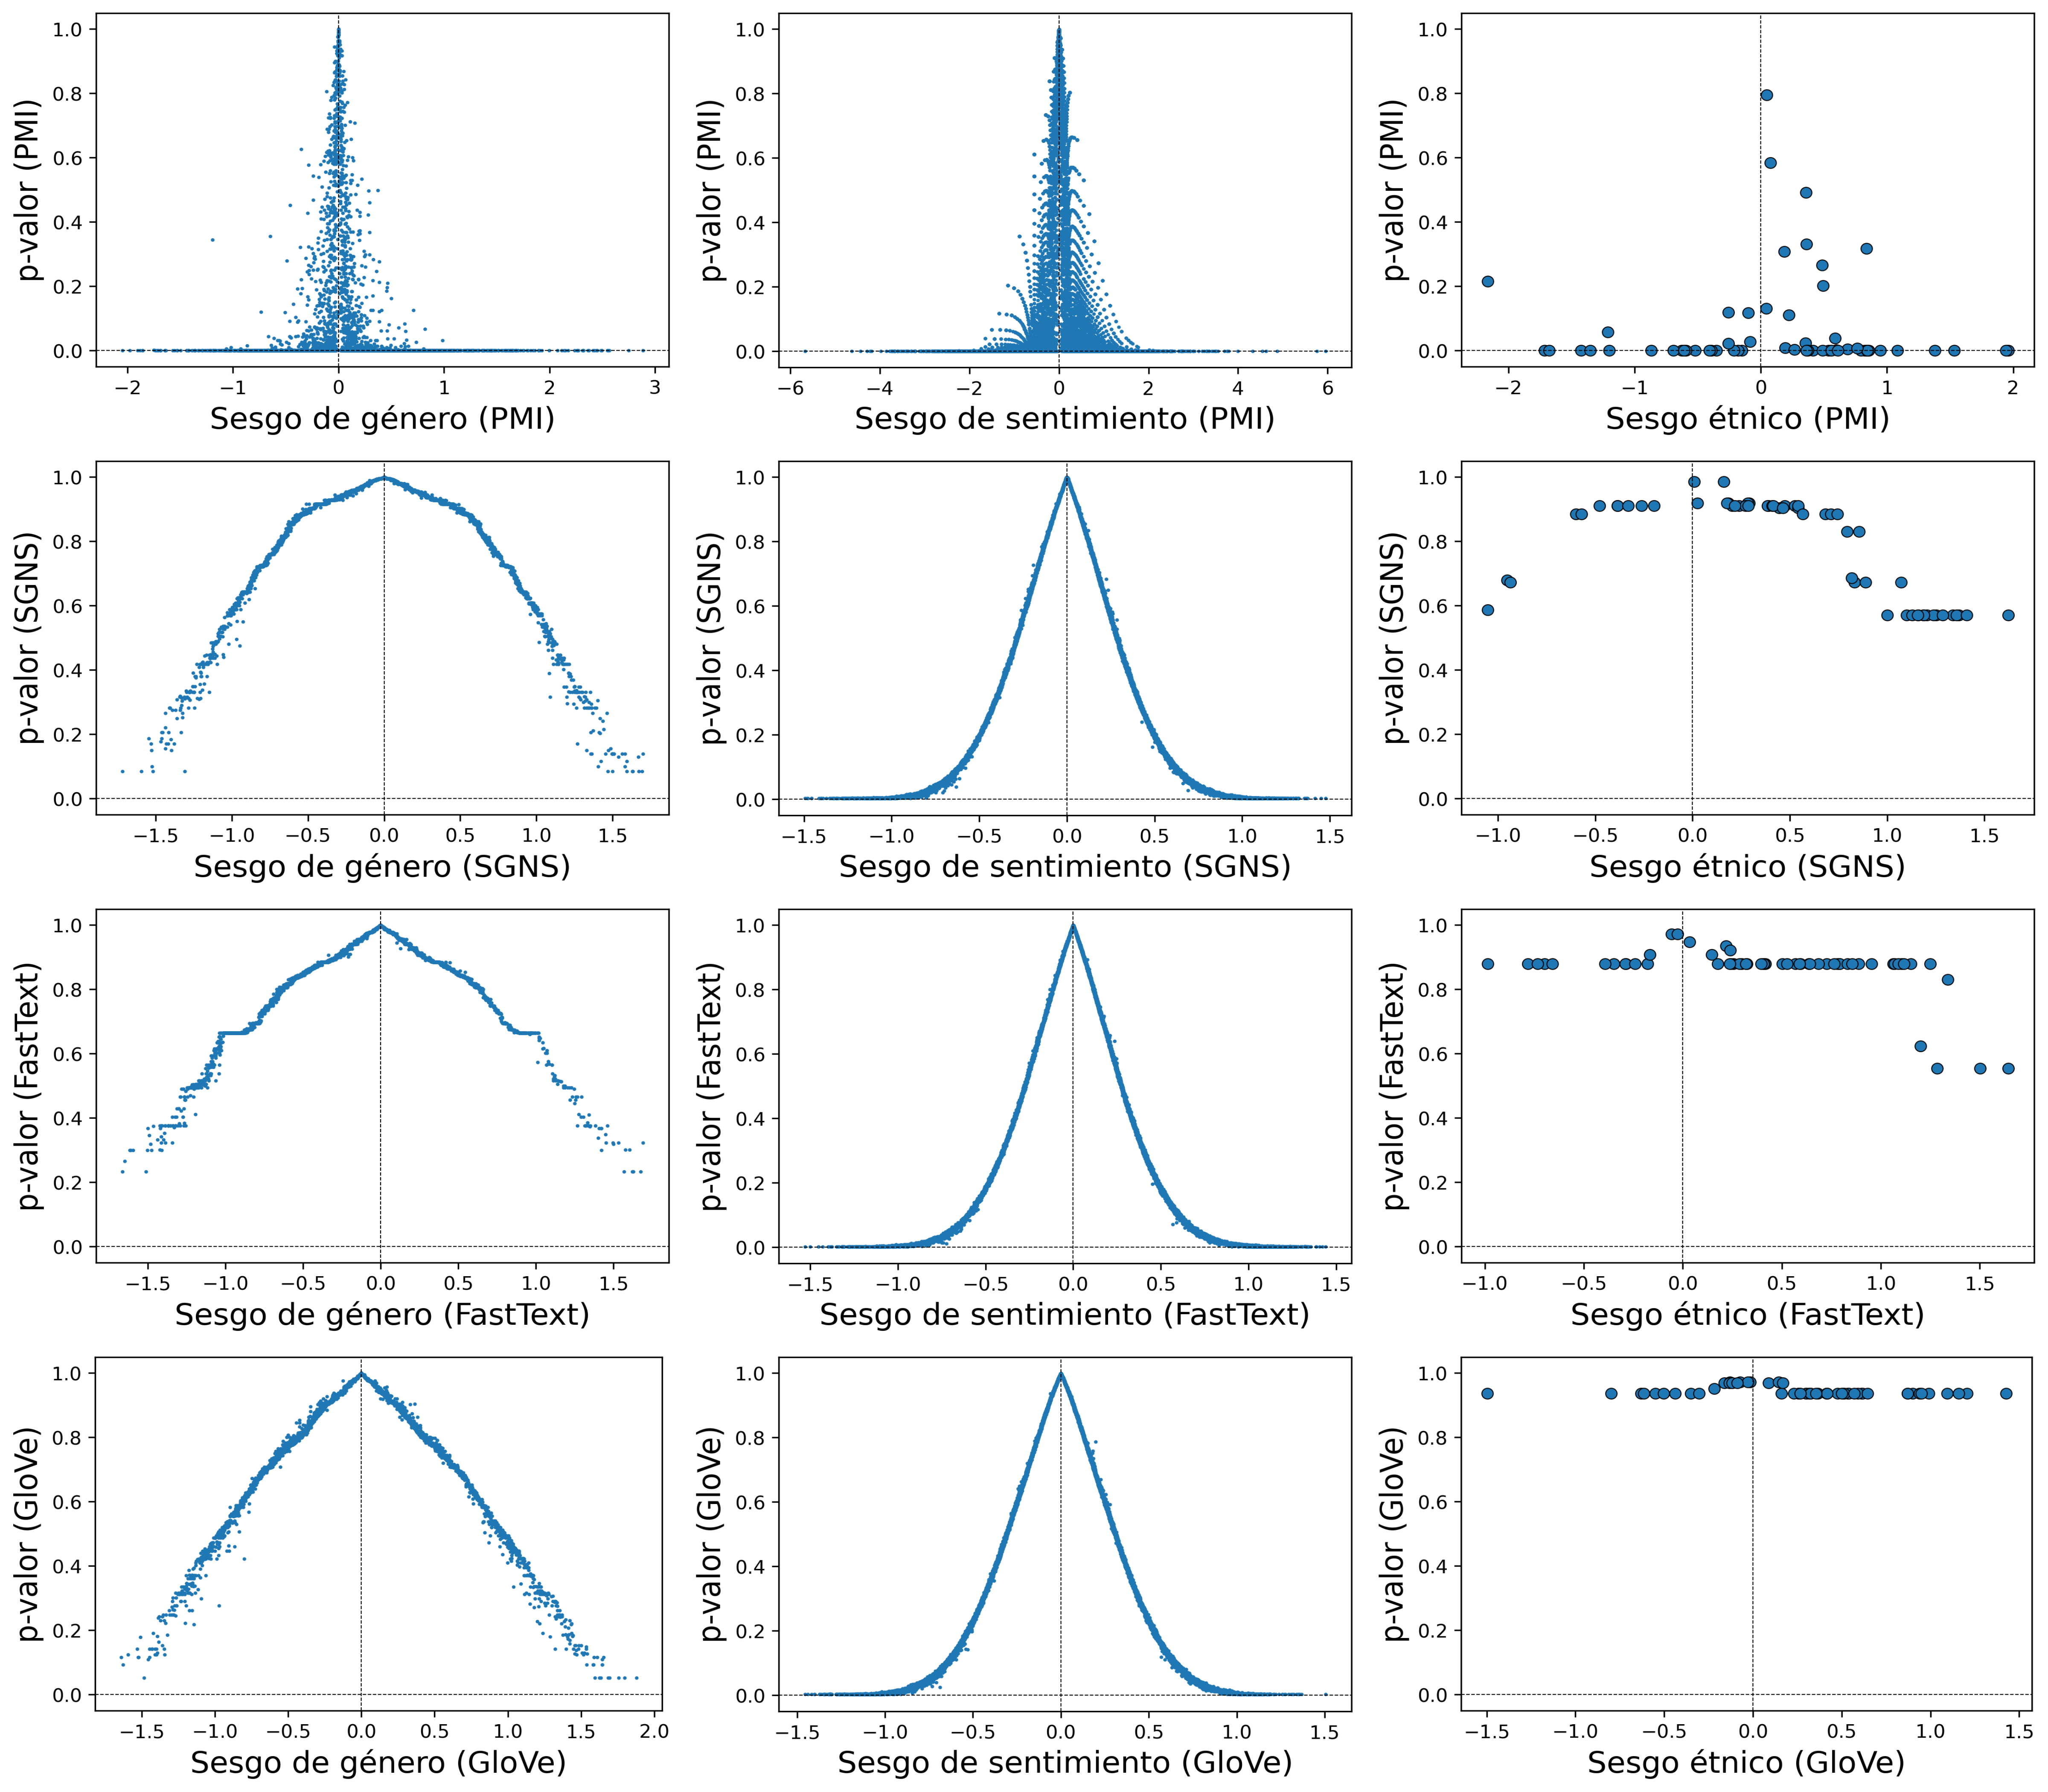
\includegraphics[width=\textwidth]{img/grid_pvalues.png}
    \caption{
        p-valores (eje vertical) en función del valor del sesgo (eje horizontal) para cada tipo de sesgo y cada método de medición.
        }
    \label{fig:pvalues}
\end{figure}


La \textbf{cantidad de palabras que se identifican con un sesgo significativamente distinto de 0 es muy distinta entre $\BiasPMI$ y $\BiasWE$} (Tabla \ref{tab:pvalues}). Por ejemplo, en el caso del sesgo de género, sólo 14 palabras de entre 4661 aparecen con $\BiasWE$ (SGNS) significativamente diferente de cero a un nivel de significatividad de 0,10, mientras que alrededor de 82\% de las palabras tienen un $\BiasPMI$ significativamente distinto de cero. Aquellas que aparecen con $\BiasPMI$ no significativo son las que tienden a tener valores de sesgo cercanos a cero (ver Figura \ref{fig:pvalues}).

Esto se debe a que \textbf{los procedimientos de cálculo de los p-valores para cada tipo de métrica capturan esencialmente distintos tipos de variabilidad}, como explicamos en la sección \ref{sec:bias_pmi_variabilidad}. La incertidumbre cuantificada para $\BiasPMI$ por medio del test de log odds ratio captura la variabilidad del proceso generador de datos subyacente, es decir, la variabilidad debida al hecho que los conteos de coocurrencias son variables aleatorias. En cambio, los p-valores de permutaciones de $\BiasWE$ sólo consideran la variabilidad de los conjuntos de palabras de contexto. 

Esta diferencia fundamental se ve reflejada en que a medida que se usan menos palabras en los grupos de contexto, la proporción de palabras que aparecen con sesgo significativamente distinto de cero es menor: alrededor de 30\% de las palabras tienen $\BiasWE$ de sentimiento significativo y ninguna palabra tiene $\BiasWE$ étnico significativo. De hecho, los p-valores de $\BiasWE$ étnico tienden a ser particularmente altos (ver Figura \ref{fig:pvalues}).  

Esta diferencia tan grande se debe a que el sesgo de sentimiento se computa con conjuntos de contexto de 25 palabras cada uno, mientras que el de etnia usa solo 4 palabras en cada grupo. En el límite, si $A$ y $B$ fueran listas de una sola palabra, no hay forma de estimar la incertidumbre para $\BiasWE$ con estos métodos, mientras que es perfectamente factible para $\BiasPMI$. Este ejemplo ilustra que estos dos métodos de inferencia miden tipos de variabilidad completamente distintos.

\begin{figure}[h]
    \centering
    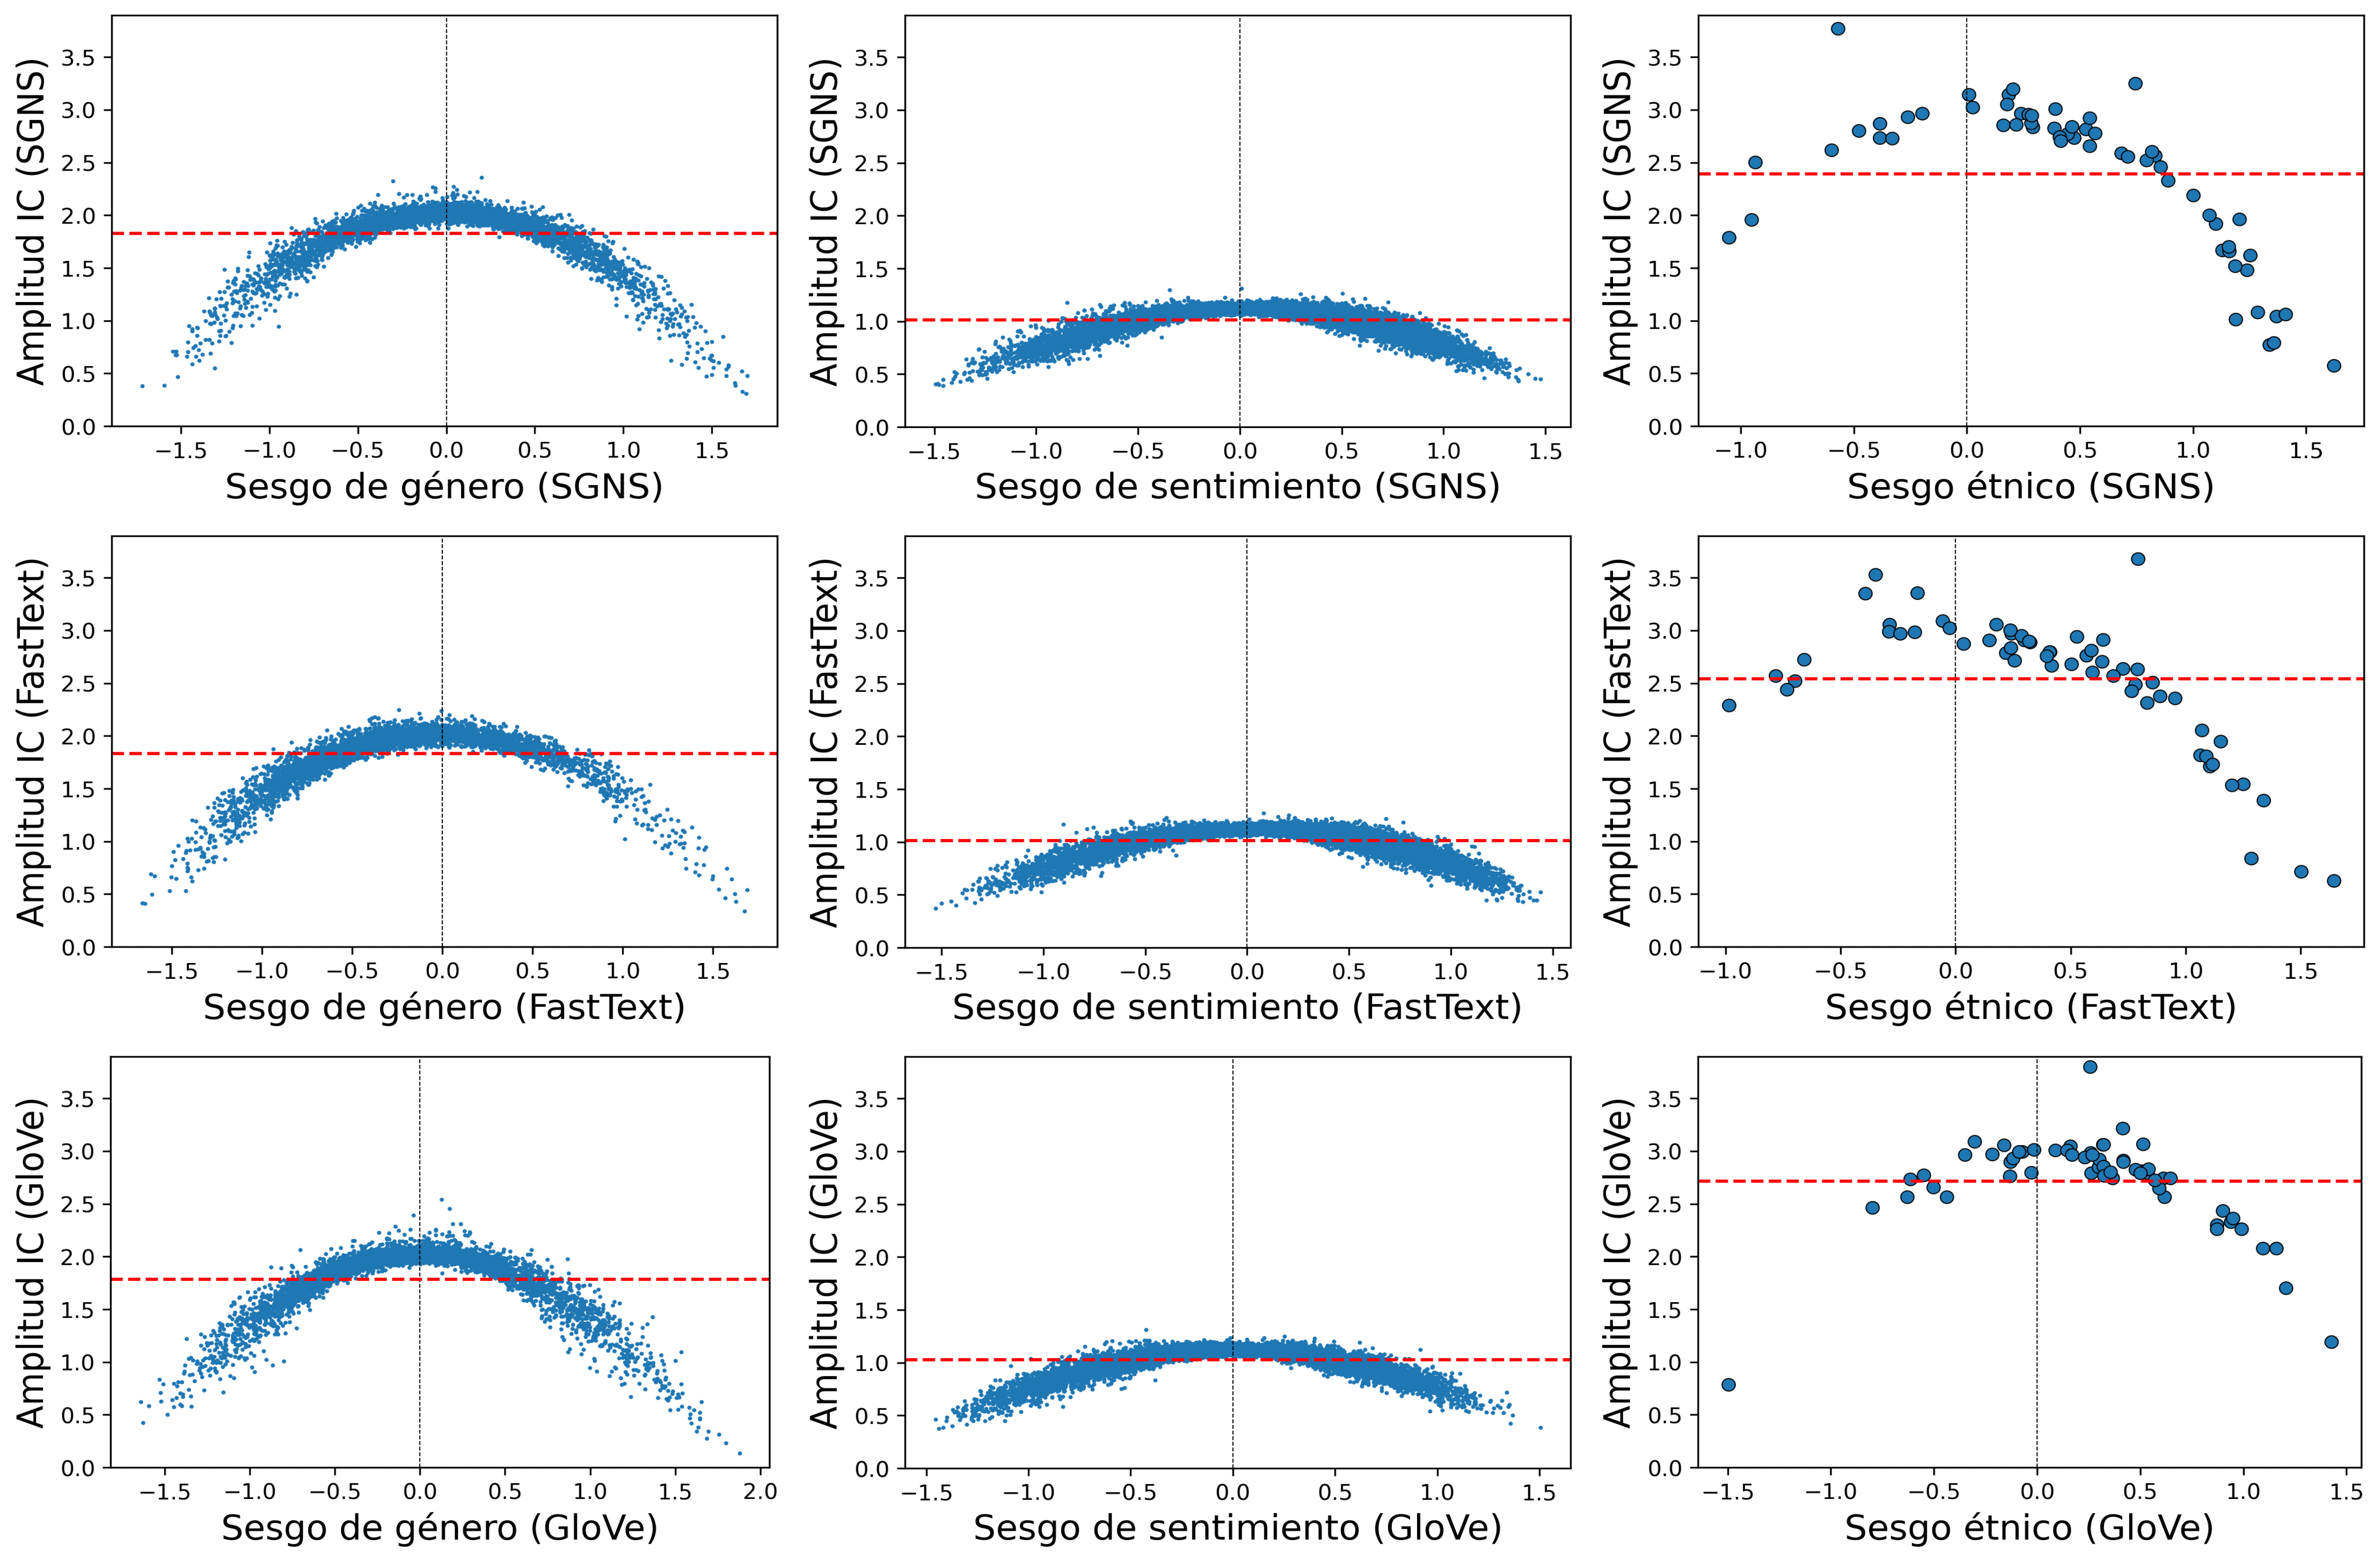
\includegraphics[width=\textwidth]{img/grid_ics.png}
    \caption{
        Amplitud de los intervalos de confianza al 95\% de $\BiasWE$ (eje vertical) en función del valor del sesgo (eje horizontal), para cada tipo de sesgo y cada método de entrenamiento de \emph{embeddings}. En rojo se indica el promedio.
        }
    \label{fig:grid_ics_bias_we}
\end{figure}

Por el mismo motivo, la \textbf{amplitud de los intervalos de $\BiasWE$} es relativamente alta en el sesgo étnico, intermedia en el sesgo de género y baja en el sesgo de sentimiento (ver Figura \ref{fig:grid_ics_bias_we}). Como hemos visto, esto no indica, por ejemplo, que haya relativamente poca evidencia a favor de que haya sesgo étnico en las palabras objetivo elegidas, sino sencillamente que estamos emepleando pocas palabras en los grupos de contexto para estimar el sesgo étnico. En cambio, las diferencias en la amplitud de los intervalos de $\BiasPMI$ sí puede atribuirse a diferencias en la evidencia disponible en el \emph{corpus} que estamos estudiando.

% NOTE la amplitud maxima del intervalo de biaswe es 4 (porque el valor max de biaswe es 2 y el min es -2)

Una de las desventajas de los métodos de estimación de la variabilidad de $\BiasWE$ es, entonces, que para detectar diferencias sistemáticas entre los grupos de contexto para una palabra objetivo determinada, requerimos listas de palabras relativamente grandes en cada grupo de contexto; pero utilizar listas más grandes, con palabras semánticamente asociadas a las palabras de contexto de interés, podría ir en detrimento de la interpretabilidad del sesgo que estamos midiendo. 

Otra ventaja del test de log odds ratios para $\BiasPMI$ es que es \textbf{computacionalmente barato} en comparación con los procedimientos de bootstrap y permutaciones requeridos para $\BiasWE$. Estos pueden ser muy lentos cuando se hace inferencia sobre muchas palabras objetivo, como es el caso de las estimaciones de sesgo de género y sentimiento en este trabajo.


Por ejemplo, para obtener los p-valores e intervalos de confianza para el conjunto de alrededor de 18,000 palabras objetivo de los tres experimentos, el tiempo de cómputo es despreciable para $\BiasPMI$, mientras que los tests de permutaciones y los intervalos de bootstrap demoran en el orden de 5 horas con el hardware que empleamos. 

Ilustramos la ventaja de $\BiasPMI$ con algunos casos individuales de medición de sesgo étnico. El $\BiasPMI$ étnico del nombre propio \emph{shanice} arroja un valor de -2,17 lo cual indica que es una palabra relativamente más asociada con \emph{white} que con \emph{black} en el corpus. Sin embargo, obtenemos un intervalo de confianza $95\%$ de $(-5,40; 1,07)$ y el p-valor para la hipótesis nula de ausencia de sesgo es de 0,20. Esto nos dice que la incertidumbre de la estimación puntual es alta y las diferencias entre \emph{A} y \emph{B} no son sistemáticas; la baja cantidad de coocurrencias en el corpus no nos permite concluir que existe un sesgo. En cambio, para la palabra \emph{wine} obtenemos $\BiasPMI = -1,71$ con IC $(-1,80; -1,62)$ y p-valor $< 10^{-10}$. En este caso podemos estar más seguros de que las coocurrencias del corpus indican que existe un sesgo étnico para \emph{wine}, que tiende a estar más asociado en primer orden con \emph{white} que con \emph{black}. 

% p-valor $< 10^{-300}$

Si usamos, en cambio, por ejemplo, $\BiasWE$ con SGNS, obtenemos $\BiasWE(shanice) = 1,07$ con IC $=(-0,19; 1,81)$ y p-valor $= 0,24$; y $\BiasWE(wine) = -0,57$ con IC $=(-1,95; 1,82)$ y p-valor $= 0,44$. Los p-valores altos e intervalos de confianza amplios que incluyen al 0 no necesariamente quieren decir que no existen sesgos sistemáticos para estas palabras en el \emph{corpus}. Por el contrario, esto ocurre porque estamos computando el sesgo con listas de palabras pequeñas que no permiten sacar conclusiones fiables acerca de la variabilidad del sesgo, como delineamos más arriba. 

% los test de permutaciones de $\BiasWE$ tienden a detectar pocos sesgos significativos


\section{Correlación con el juicio humano} \label{sec:experimento_correlacion}

Para los tres sesgos que analizamos, evaluamos la \textbf{correlación entre las métricas de sesgo textual y el sesgo de acuerdo al juicio humano}. Medimos la correlación con el coeficiente \emph{r} de Pearson. También calculamos un \emph{r} de Pearson ponderado, que tiene en cuenta el error estándar de cada estimación de sesgo textual y reduce la influencia de las estimaciones ruidosas en la correlación. 

El objetivo de este experimento no es encontrar qué método produce mayores correlaciones, sino más bien estudiar si los resultados de $\BiasPMI$ son similares a los de $\BiasWE$, de uso más difundido en este tipo de análisis. 



\begin{table}[h]
  \centering
  \begin{tabular}{lccccc}
    \toprule
    Sesgo                                    & Correlación   & PMI                & SGNS & FastText & GloVe              \\
    \midrule
    \multirow[c]{2}{*}{Sesgo de género}      & $r$           & 0.51               & 0.49 & 0.47     & 0.46               \\
                                             & $r$ ponderado & 0.45               & 0.62 & 0.63     & 0.69               \\
    \cline{1-6}
    \multirow[c]{2}{*}{Sesgo de sentimiento} & $r$           & 0.43               & 0.59 & 0.59     & 0.58               \\
                                             & $r$ ponderado & 0.34               & 0.66 & 0.66     & 0.64               \\
    \cline{1-6}
    \multirow[c]{2}{*}{Sesgo étnico}         & $r$           & {\color{gray}0.14} & 0.44 & 0.36     & {\color{gray}0.30} \\
                                             & $r$ ponderado & 0.15               & 0.51 & 0.20     & {\color{gray}0.43} \\
    \cline{1-6}
    \bottomrule
  \end{tabular}
  \caption[Coeficientes de correlación de Pearson entre el sesgo de acuerdo al juicio humano y el sesgo textual medido con cada métrica]{
    Coeficientes de correlación de Pearson entre el sesgo de acuerdo al juicio humano y el sesgo textual medido con cada métrica. Los coeficientes son significativos con un nivel de confianza superior 99\%, exceptuando el $r$ y el $r$ ponderado de GloVe para el sesgo étnico, y el $r$ de PMI para el sesgo étnico, los cuales tienen p-valores $> 0,10$.
  }
  \label{tab:correlaciones}
\end{table}


% \begin{tabular}{llrrrr}
%   \toprule
%                                            &               & PMI  & SGNS & FastText & GloVe \\
%   Sesgo                                    & Correlación   &      &      &          &       \\
%   \midrule
%   \multirow[c]{2}{*}{Sesgo de género}      & $r$           & 0.51 & 0.49 & 0.47     & 0.46  \\
%                                            & $r$ ponderado & 0.45 & 0.62 & 0.63     & 0.69  \\
%   \cline{1-6}
%   \multirow[c]{2}{*}{Sesgo de sentimiento} & $r$           & 0.43 & 0.59 & 0.59     & 0.58  \\
%                                            & $r$ ponderado & 0.34 & 0.66 & 0.66     & 0.64  \\
%   \cline{1-6}
%   \multirow[c]{2}{*}{Sesgo étnico}         & $r$           & 0.14 & 0.44 & 0.36     & 0.30  \\
%                                            & $r$ ponderado & 0.15 & 0.51 & 0.20     & 0.43  \\
%   \cline{1-6}
%   \bottomrule
% \end{tabular}


\begin{figure}[H]
    \centering
    \includegraphics[width=0.85\textwidth]{img/grid_glasgow-gender.png}
    \caption{
        Relación entre el sesgo de género textual y de acuerdo al juicio humano en las palabras de \citet{lewis2020gender}. Cada punto representa una palabra objetivo. Las rectas representan un ajuste lineal de los datos. En la segunda fila el ajuste pondera cada punto por el error estándar de la estimación de sesgo textual (los intervalos de confianza asociados no se muestran para mayor claridad).
    }
    \label{fig:grid_corr_genero}
\end{figure}

\begin{figure}[H]
    \centering
    \includegraphics[width=0.85\textwidth]{img/grid_warriner-valence.png}
    \caption{
        Relación entre el sesgo de sentimiento textual y de acuerdo al juicio humano en las palabras de \citet{toney2021valnorm}. Cada punto representa una palabra objetivo. Las rectas representan un ajuste lineal de los datos. En la segunda fila el ajuste pondera cada punto por el error estándar de la estimación de sesgo textual (los intervalos de confianza asociados no se muestran para mayor claridad).
    }
    \label{fig:grid_corr_sentimiento}
\end{figure}

\begin{figure}[H]
    \centering
    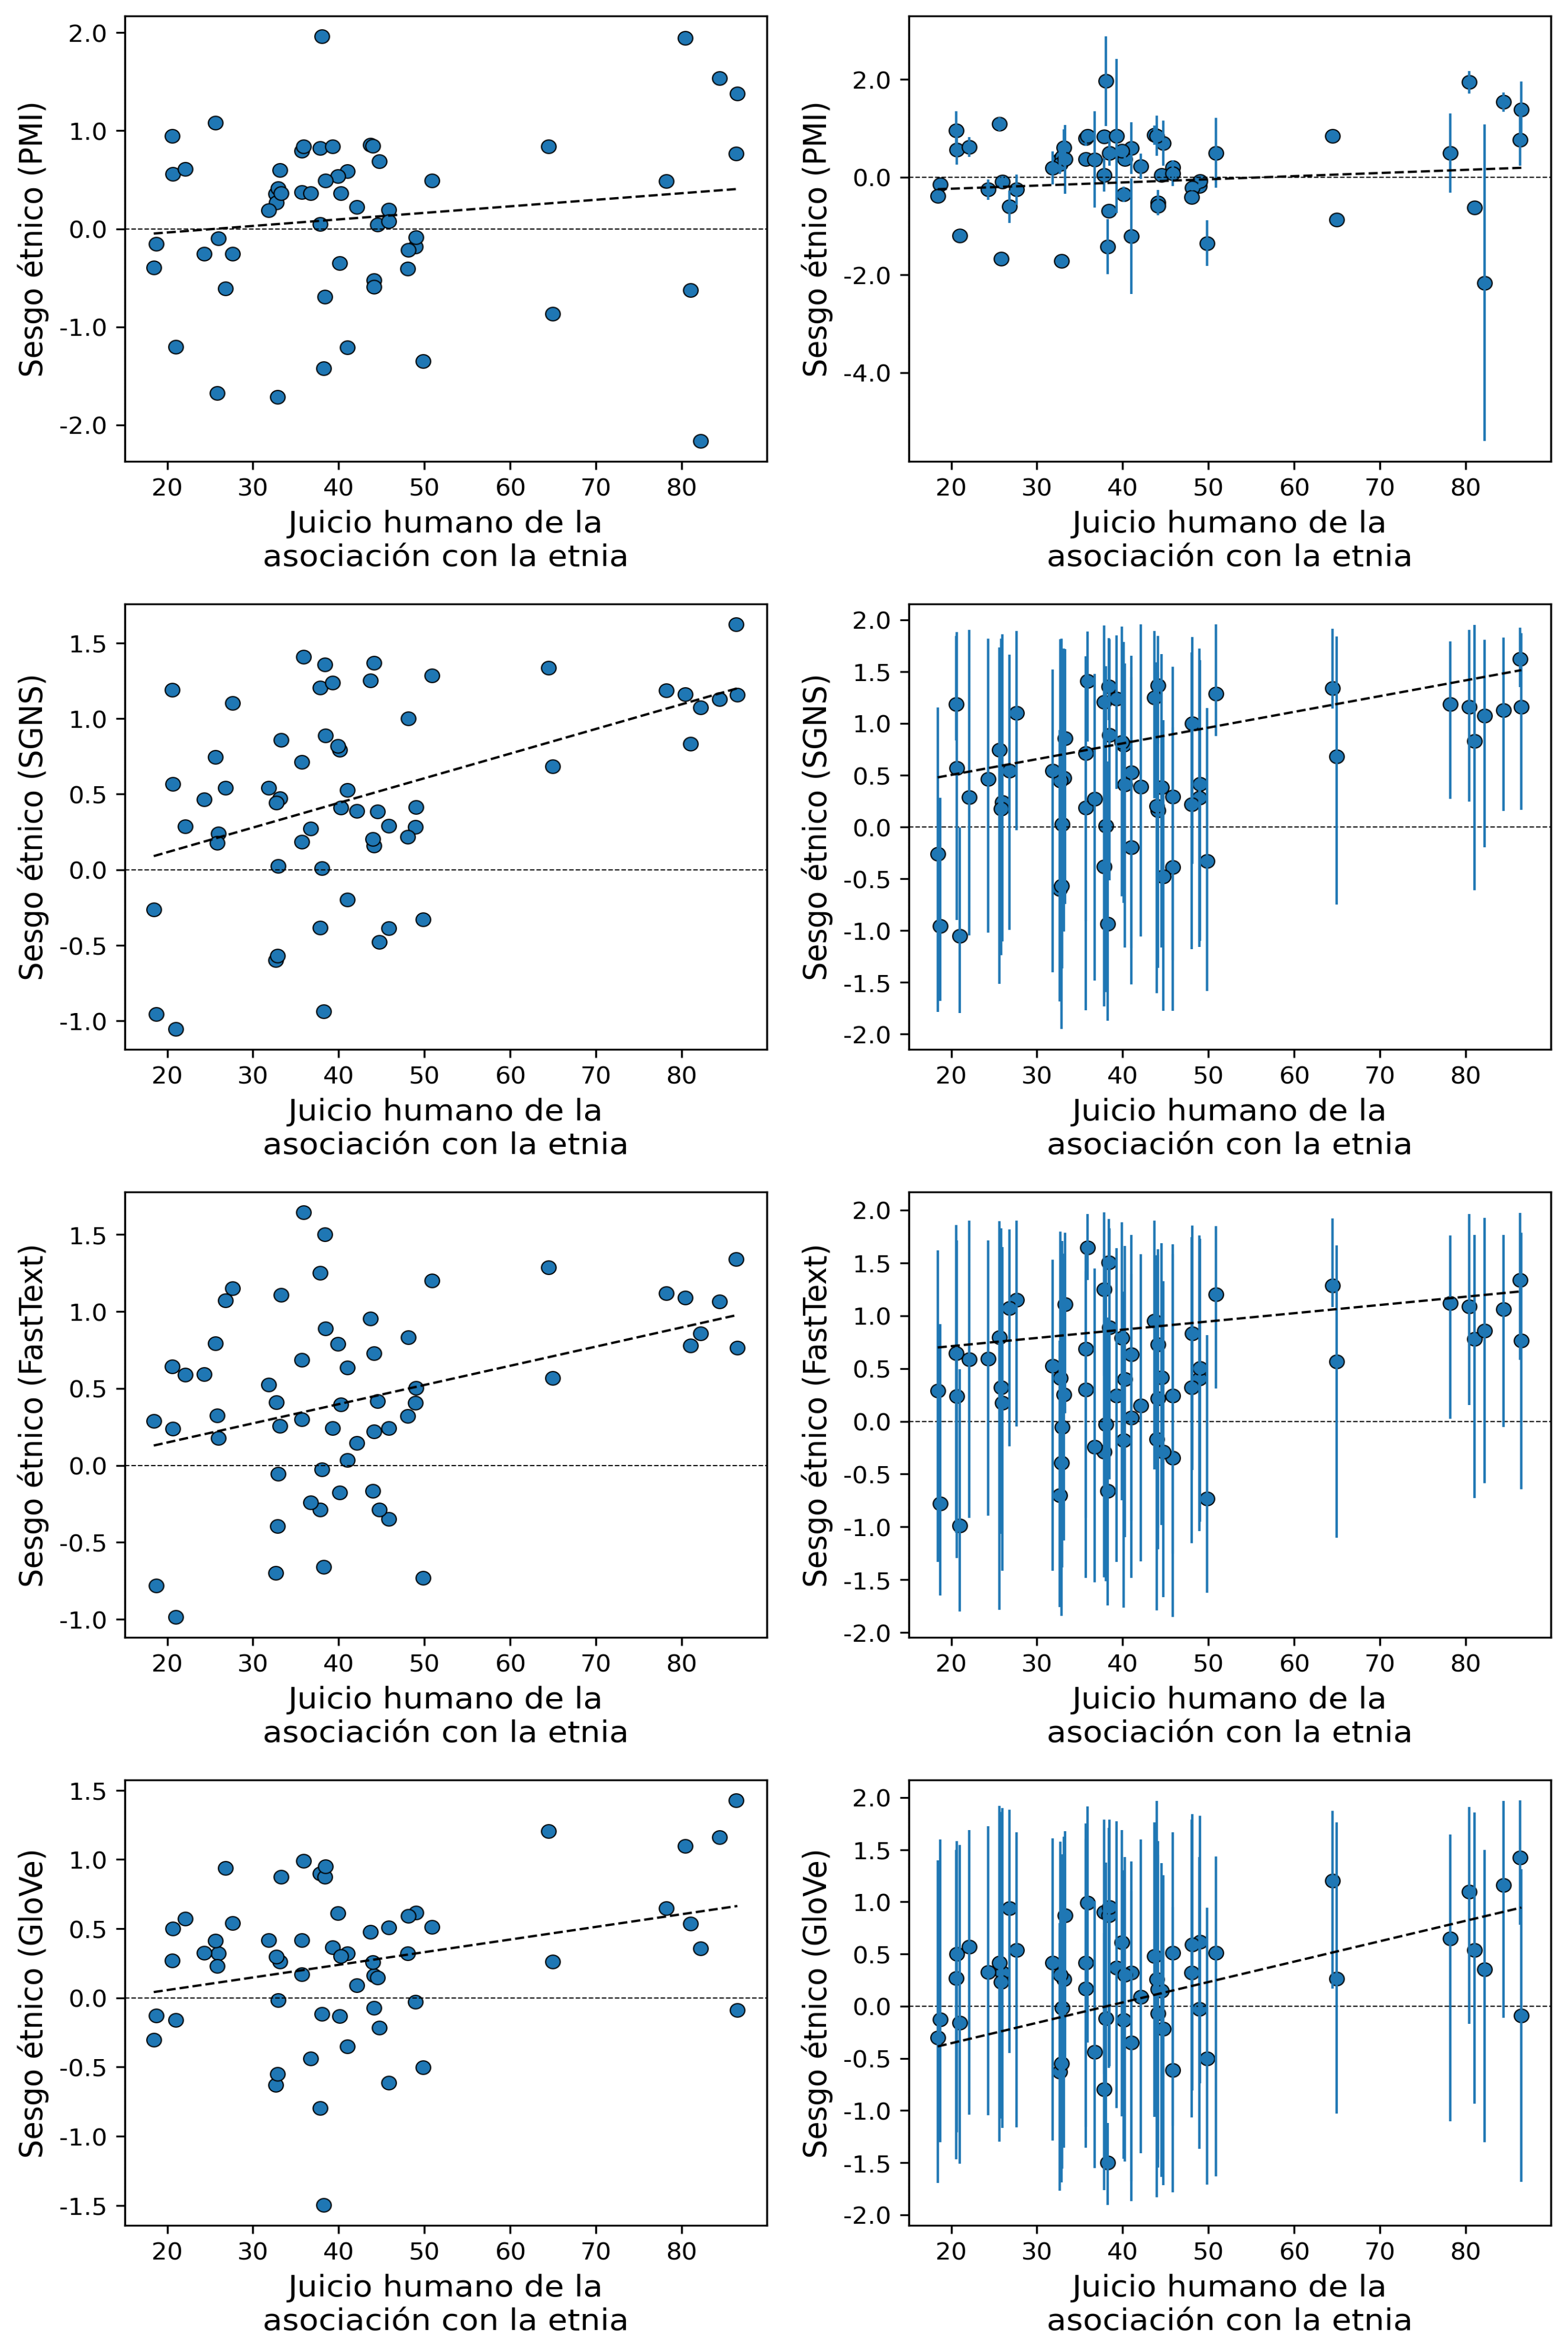
\includegraphics[width=0.85\textwidth]{img/grid_mturk-race.png}
    \caption{
        Relación entre el sesgo étnico textual y de acuerdo al juicio humano en las palabras de \citet{kozlowski2019geometry}. Cada punto representa una palabra objetivo. Las rectas representan un ajuste lineal de los datos. En la segunda fila el ajuste pondera cada punto por el error estándar de la estimación de sesgo textual (los intervalos de confianza se indican con barras de error).
    }
    \label{fig:grid_corr_etnico}
\end{figure}


Encontramos \textbf{correlaciones positivas entre todas las métricas de sesgo textual y los sesgos de acuerdo al juicio humano} (ver la Tabla \ref{tab:correlaciones} con los coeficientes de correlación; los diagramas de dispersión asociados se encuentran en las Figuras \ref{fig:grid_corr_genero}, \ref{fig:grid_corr_sentimiento} y \ref{fig:grid_corr_etnico}). Esto es consistente con los hallazgos previos de los estudios en los cuales están basados los tres experimentos \citep{lewis2020gender,kozlowski2019geometry,toney2021valnorm}, los cuales usan métricas de sesgo textual basadas en \emph{word embeddings}.

También hallamos que, en general, el uso de ponderadores para calcular la correlación aumenta los coeficientes de $\BiasWE$. Esto implica que reducir la ponderación de estimaciones más ruidosas (donde la diferencia de similitudes con respecto a las listas de palabras $A$ y $B$ no es tan sistemática) tiende a incrementar la correlación del sesgo de este \emph{corpus}. En cambio, los coeficientes de correlación de $\BiasPMI$ tienden a caer o permanecer constantes cuando se usan ponderadores, lo cual indica que los pesos tienden a ser mayores en palabras donde el sesgo textual estimado no coincide con el sesgo de acuerdo al juicio humano. No tenemos ninguna hipótesis sobre por qué el efecto de usar ponderadores es distinto para $\BiasWE$ y $\BiasPMI$.

Remarcamos que esto no significa que para cada estimación individual de sesgo los errores estándar de cada método sean mutuamente intercambiables o igualmente útiles, dado que capturan tipos de variabilidad distinta (ver secciones \ref{sec:bias_pmi_variabilidad} y \ref{sec:experimento_variabilidad}). Esto se ve reflejado en que los intervalos de confianza de $\BiasWE$ tienden a ser relativamente más anchos en $\BiasWE$ que en $\BiasPMI$, como se observa en la Figura \ref{fig:grid_corr_etnico}. 

Tomando como referencia el coeficiente de correlación más alto de cada tipo de métrica ($\BiasPMI$ vs. $\BiasWE$) en cada sesgo, se obtienen correlaciones más altas con $\BiasWE$ que con $\BiasPMI$. La diferencia es particularmente alta en el caso del sesgo étnico ($\max(r_{\BiasWE})=0.51$ vs. $\max(r_{\BiasPMI})=0.15$), donde además el grado de correlación de $\BiasPMI$ es especialmente débil. 

Una hipótesis que puede explicar este resultado es que en este estereotipo las \textbf{asociaciones de segundo orden} juegan un rol importante, y éstas no son capturadas por $\BiasPMI$. Determinados consumos culturales como el \emph{basketball} pueden estar más asociados a \emph{black} que a \emph{white} no porque \emph{basketball} aparezca relativamente más en el contexto de palabras que explícitamente refieren a \emph{black} (las palabras de contexto), sino porque comparten vecinos en común, como pueden ser los nombres de las personas que juegan al basketball.

Este tipo de asociación puede ser capturada por los puntajes de juicio humano y por $\BiasWE$, pero no necesariamente por $\BiasPMI$. Una manera de capturar esto con $\BiasPMI$ puede ser extendiendo las listas de palabras de contexto, por ejemplo con nombres propios o apellidos típicos de cada etnia (como se realiza, por ejemplo, en \citet{garg2018word}). En la sección \ref{sec:experimento_interpretabilidad} discutimos con mayor detalle las diferencias entre $\BiasPMI$ y $\BiasWE$ en términos de los tipos de asocaciones semánticos y aspectos del \emph{corpus} que capturan.  

Enfatizamos que no consideramos que los coeficientes de correlación con el juicio humano (Tabla \ref{tab:correlaciones}) sean una medida de la bondad global de una métrica de sesgo. El objetivo de nuestro análisis es analizar en qué medida los resultados que se obtienen con los dos tipos de métricas son similares. Con otras listas de palabras probablemente se obtengan otros resultados. Asimismo, es probable que Wikipedia no sea necesariamente representativa de los estereotipos sociales codificados en los puntajes de las encuestas que se usan en cada experimento. Incorporar \emph{corpora} de otros dominios podría dar lugar a correlaciones mayores o menores. 

Por otra parte, hasta donde sabemos, no existen \emph{corpora} anotados con los sesgos que contienen. Disponer de ese \emph{ground truth} sería valioso para la tarea de medir sesgos en textos porque permitiría evaluar las métricas de manera más directa, comparando el sesgo textual estimado con el sesgo anotado. Sin embargo, no es obvio cómo anotar la cantidad de sesgo de una palabra en un \emph{corpus}, particularmente si el \emph{corpus} es grande. En los tres experimentos que estudiamos, las ``anotaciones'' son promedios de valoraciones de humanos sobre la semántica de las palabras, y no tienen en cuenta ningún \emph{corpus} en particular. La falta de estas etiquetas hace que no esté claro cómo sacar conclusiones sobre si un método es globalmente mejor que otro a la hora de medir el sesgo en palabras específicas de un texto.


\section{Interpretación de las estimaciones} \label{sec:experimento_interpretabilidad}

En esta sección, analizamos las ventajas y desventajas de medir los sesgos con \emph{word embeddings} en comparación a una métrica de asociación de primer orden como $\BiasPMI$. En particular, usaremos ejemplos concretos de mediciones de sesgo de género binario para \textbf{comparar la interpretación de las estimaciones con cada método}.

Como hemos visto en la sección \ref{sec:bias_pmi}, $\BiasPMI$ puede expresarse intrínsecamente en términos de probabilidades condicionales (ecuación \ref{eq:bias_pmi_condicional}). El sesgo se interpreta en este caso como el logaritmo de cuánto más probable es encontrar palabras de $C$ en el contexto de palabras en $A$ que en el contexto de palabras en $B$. Dado que \textbf{$\BiasPMI$ puede interpretarse de forma transparente en términos de coocurrencias de primer orden}, podemos decir que $\BiasPMI$ es una métrica absoluta que no requiere comparaciones con otros sesgos para ser interpretada. 

Podemos ilustrar esta propiedad con un ejemplo individual. Cuando medimos el sesgo de género binario (femenino/masculino) en el \emph{corpus} de Wikipedia, obtenemos que $\BiasPMI(nurse)$ $\approxeq
1,3172$. Por lo tanto,
%
\begin{equation*}
    \frac{P(nurse|A)}{P(nurse|B)} \approxeq
    e^{1,3172} \approxeq
    3,7330.
\end{equation*}
%
Esto significa que es aproximadamente un 273,30 \% más probable encontrar la palabra \emph{nurse} en el contexto de palabras femeninas ($A$) que en el contexto de palabras masculinas ($B$).

En el caso de $\BiasWE$, si bien existen estudios que buscan interpretar cómo se forman los espacios vectoriales de los \emph{embeddings} \citep{levy2014neural,levy2015improving,ethayarajh2019understanding} o que analizan los patrones semánticos que codifican \citep{bolukbasi2016man,zhao2017men,gonen2019lipstick}, no existe una interpretación transparente de las métricas de sesgo basadas en \emph{embeddings} en términos de las coocurrencias de palabras en los textos.

Esta falta de interpretabilidad de $\BiasWE$ se debe a que la similitud entre \emph{embeddings} como SGNS, GloVe y FastText puede captar asociaciones entre palabras tanto de primer orden (sintagmáticas) como de segundo orden (paradigmáticas) o superior \citep{altszyler2018corpus,schlechtweg2019second}. Entonces, cuando usamos \emph{embeddings} para medir sesgos, no es posible saber si los resultados se deben a coocurrencias de primer orden generalizadas o se derivan de coocurrencias de orden superior poco transparentes \citep{brunet2019understanding,rekabsaz2021measuring}. En definitiva, mientras \textbf{la relación entre $\BiasWE$ y la distribución de palabras no es transparente}, en el caso de $\BiasPMI$ sí lo es porque $\PMI$ es estrictamente una métrica de asociación de primer orden.

% NOTE estos valores en realidad son de OpenSubs pero puse Wiki porque no usé OpenSubs en la tesis (:

Ejemplificamos esta diferencia en interpretabilidad con el caso de la palabra \emph{evil}. En Wikipedia, el $\BiasPMI$ de género de \emph{evil} es igual a $-0,25$, lo que indica una mayor probabilidad de aparecer en el contexto de palabras de contexto masculino ($B$) en comparación con las femeninas ($A$). Por el contrario, $\BiasWE=0,23$ con SGNS. Aunque sabemos que esto se interpreta como un sesgo femenino, es difícil comprender el origen exacto de este resultado porque está influido por coocurrencias de segundo orden o superior, y no podemos medir el peso que tiene cada uno de estos factores. 

A continuación mostramos otros ejemplos que ilustran cómo el orden de asociación puede influir en las estimaciones de sesgo de género:

\begin{itemize}

    % NOTE estos valores en realidad son de OpenSubs pero puse Wiki porque no usé OpenSubs en la tesis (:
    \item Hay palabras no incluidas en el grupo $A$ que intrínsecamente tienen un sesgo femenino, como \emph{women}, \emph{wife}, \emph{ladies} o \emph{girls}. Sin embargo, estas palabras aparecen con $\BiasPMI < 0$ (sesgo masculino) porque tienden a aparecer relativamente más en el contexto de palabras masculinas (grupo $B$) que femeninas (grupo $A$) en Wikipedia (por ejemplo, \emph{his wife}). Probablemente la asociación de estas palabras con las del grupo $A$ sea de segundo orden o paradigmática (tienden a tener vecinos similares), y este aspecto no es capturado por $\BiasPMI$.
    
    % NOTE estos valores en realidad son de OpenSubs pero puse Wiki porque no usé OpenSubs en la tesis (:
    \item Ocupaciones como \emph{assistant} y \emph{secretary} están estereotípicamente asociadas al género femenino \citep{caliskan2017semantics}. Sin embargo, obtenemos valores de $\BiasPMI$ de género de $-0,19$ y $-0,24$,  respectivamente (ambos con p-valor $< 10^{-5}$). Esto indica una asociación de primer orden más fuerte con las palabras de contexto masculinas ($B$) en comparación con las femeninas ($A$); por ejemplo, por la presencia de estructuras como \emph{his assistant}. Al usar $\BiasWE$ con SGNS obtenemos valores de $0,70$ y $0,43$, respectivamente: el sesgo invierte su signo. Esto podría deberse al efecto de la asociación de segundo orden: estas palabras probablemente tienen vecinos similares a las palabras del grupo $A$, es decir, aparecen en contextos similares (por ejemplo, contextos relacionados a la oficina o el cuidado).
    
    % NOTE esto sí es de wiki:
    \item Palabras como \emph{harbor}, \emph{navy}, \emph{dock}, \emph{port}, \emph{fleet}, \emph{steam}, \emph{pier}, \emph{sailor}, \emph{ship}, y \emph{sail} tienen valores positivos de $\BiasPMI$ de género en Wikipedia. Esto puede deberse a que en el idioma inglés, los barcos se suelen denominar con pronombres femeninos como \emph{she}. Los valores de $\BiasWE$ con SGNS para estas palabras son, en cambio, inferiores a 0, posiblemente porque estas palabras están más relacionadas con el género masculino a través de coocurrencias de segundo orden (e.g. los barcos y los varones pueden aparecer en contextos similares relacionados a la marina o la guerra).

\end{itemize}

Otro aspecto interesate a considerar es que las métricas de sesgo que capturan asociaciones de segundo orden tienen la ventaja de \textbf{gestionar la \emph{raleza} de los datos (\emph{data sparsity})}. Dado que todo \emph{corpus} es limitado, algunas de las muchas formas que pueden tomar los conceptos objetivo y de contexto pueden aparecer raramente en el texto. En este escenario en el que las coocurrencias son ralas (\emph{sparse}), cuando usamos $\BiasWE$, puede que no sea necesario incluir todas las palabras relacionadas con los conceptos objetivo y de contexto para medir sesgos exitosamente, dado que los \emph{embeddings} pueden captar sinonimia. En el caso de $\BiasPMI$, este problema debe abordarse aumentando las listas de palabras con sinónimos y formas de las palabras de interés.

Para ejemplificar esto, consideremos el caso de los sinónimos \emph{nourish} y \emph{nurture}, que tienen frecuencias diferentes en el corpus de Wikipedia ($700$ y $3,000$, respectivamente). Con $\BiasPMI$, obtenemos un sesgo de $0,33$ para \emph{nurture} (p-valor $< 10^{-4}$). Sin embargo, si hubiéramos utilizado en su lugar su sinónimo menos frecuente \emph{nourish}, el $\BiasPMI$ habría sido $-0,10$ y no habría sido estadísticamente significativo (p-valor $\approx 0,66$). En este caso no habríamos podido determinar si realmente no hay sesgo o si la cantidad de datos es insuficiente para determinar esto. 

Esto demuestra que, en general, es aconsejable incluir todos los sinónimos y variaciones pertinentes del término cuyo sesgo intentamos medir cuando usamos $\BiasPMI$. Por otra parte, cuando se usa $\BiasWE$ podríamos confiar en el hecho de que los \emph{embeddings} pueden capturar sinonimia; en este ejemplo particular $\BiasWE$ con SGNS arroja valores positivos para ambas palabras.

Por último, en investigaciones recientes hemos demostrado que \textbf{$\BiasWE$, a diferencia de $\BiasPMI$, puede producir resultados engañosos porque captura inadvertidamente las disparidades en las frecuencias de las palabras de contexto} \citep{valentini2022undesirable}. 

Para dar cuenta de este problema en el contexto de la interpretabilidad, analizamos las estimaciones de sesgo de \emph{stopwords}, es decir, palabras muy frecuentes con poco contenido semántico (ver Tabla \ref{tab:stopwords}). Mientras que $\BiasPMI$ no tiende a detectar sesgo de género sistemáticamente en alguna dirección en las \emph{stopwords}, $\BiasWE$ con cualquiera de los tres métodos de generación de \emph{embeddings} tiende a producir estimaciones de sesgo siempre negativas i.e. con sesgo masculino. Esto se debe a que las palabras de contexto masculinas (grupo $B$) son más frecuentes que las femeninas (grupo $A$) en el corpus de Wikipedia, y a que los \emph{embeddings} tienen la capacidad de capturar la frecuencia de las palabras \citep
{valentini2022undesirable}. 



\begin{table}[h]
  \centering
  \begin{tabular}{lrrrr}
    \toprule
    Palabra & PMI   & SGNS  & FastText & GloVe \\
    \midrule
    which   & -0.08 & -0.50 & -0.59    & -0.51 \\
    first   & 0.03  & -0.15 & -0.28    & -0.50 \\
    after   & -0.06 & -0.60 & -0.73    & -0.62 \\
    have    & 0.13  & -0.42 & -0.35    & -0.45 \\
    other   & 0.07  & -0.57 & -0.45    & -0.44 \\
    all     & -0.05 & -0.55 & -0.58    & -0.64 \\
    over    & -0.20 & -0.80 & -0.87    & -0.76 \\
    only    & 0.02  & -0.46 & -0.56    & -0.60 \\
    most    & -0.13 & -0.53 & -0.56    & -0.62 \\
    up      & 0.11  & -0.63 & -0.67    & -0.64 \\
    used    & -0.13 & -0.72 & -0.38    & -0.68 \\
    under   & -0.16 & -0.96 & -1.12    & -1.15 \\
    part    & 0.07  & -0.31 & -0.41    & -0.40 \\
    many    & -0.15 & -0.42 & -0.60    & -0.64 \\
    well    & 0.04  & -0.29 & -0.44    & -0.52 \\
    name    & 0.13  & -0.26 & -0.28    & -0.50 \\
    several & -0.09 & -0.36 & -0.53    & -0.53 \\
    same    & 0.05  & -0.06 & -0.40    & -0.54 \\
    former  & -0.21 & -0.60 & -0.59    & -0.59 \\
    system  & -0.55 & -1.01 & -0.77    & -0.93 \\
    \bottomrule
  \end{tabular}
  \caption{
    Sesgo de género de las 20 \emph{stopwords} más frecuentes de las palabras del experimento de Glasgow \citep{scott2019glasgow}.
  }
  \label{tab:stopwords}
\end{table}



En consecuencia, no podemos interpretar qué aspectos del corpus dan lugar a las estimaciones de sesgo que observamos. Cuando usamos $\BiasWE$, en definitiva, no solo es dificil determinar el tipo de asociación que da origen a los resultados, sino también si el sesgo semántico detectado es genuino o si sólo se debe a la disparidad en las frecuencias de las palabras de contexto.



\chapter{Conclusiones} \label{cap:conclusiones}

En los últimos años, la temática de los sesgos en los modelos de aprendizaje automático ha suscitado una gran atención. Aunque numerosos estudios han explorado los sesgos presentes en los modelos, siguen siendo escasas las herramientas diseñadas para medir y analizar directamente los sesgos en los textos. Además, estas herramientas suelen carecer de interpretabilidad. En esta tesis, abordamos estas deficiencias introduciendo y analizando una métrica basada en \emph{Pointwise Mutual Information} (PMI) para medir sesgos en \emph{corpora}. A través de nuestra investigación, hemos destacado las diferencias del enfoque basado en PMI sobre las métricas tradicionales basadas en \emph{word embeddings} estáticos, como SGNS, GloVe y FastText, poniendo especial énfasis en las ventajas.

%A través de nuestra investigación, hemos hecho varias contribuciones importantes y destacado las ventajas del enfoque basado en PMI sobre las métricas tradicionales basadas en \emph{word embeddings} estáticos, como SGNS, GloVe y FastText.

Una de las principales contribuciones de nuestro trabajo es la introducción de la métrica basada en PMI como \textbf{método sencillo, interpretable y computacionalmente efeciente de medir sesgos textuales}. A diferencia de las métricas basadas en \emph{embeddings}, que carecen de transparencia e interpretabilidad, nuestro enfoque ofrece una interpretación clara en términos de coocurrencias de primer orden, y por lo tanto, una comprensión más intuitiva de los sesgos subyacentes presentes en los textos.

Además, introducimos una \textbf{técnica paramétrica para estimar la incertidumbre asociada a las estimaciones} de la métrica basada en PMI. Esta manera de medir la variabilidad permite a los investigadores determinar hasta qué punto los valores medidos pueden atribuirse a fluctuaciones estadísticas. A diferencia de las metodologías tradicionales basadas en el remuestreo, como el \emph{bootstrapping} y las pruebas de permutación utilizadas habitualmente con los \emph{embeddings}, nuestro enfoque paramétrico brinda una estimación más informativa de la verdadera variabilidad en las mediciones de sesgo.

Mediante una serie de experimentos, presentamos \textbf{evidencia empírica que respalda las ventajas del método basado en PMI} frente a las métricas basadas en \emph{embeddings}. Estos resultados demuestran, asimismo, que la métrica basada en PMI muestra asociaciones similares con el juicio humano que las métricas basadas en \emph{embeddings} en determinados escenarios, como los sesgos de género; mientras que en otros casos, como los estereotipos étnicos, PMI y \emph{embeddings} arrojan resultados divergentes. Esta distinción subraya las diferencias fundamentales en las asociaciones semánticas capturadas por los \emph{embeddings} y PMI, respectivamente.

La disponibilidad de herramientas para medir sesgos en los textos es limitada, y la interpretabilidad de estas herramientas es aún más acotada. Nuestro trabajo aborda esta necesidad proporcionando un método transparente e interpretable. Creemos que los estudios centrados en la interpretabilidad y las propiedades estadísticas de las métricas son de suma importancia para el NLP. Al facilitar análisis más transparentes e interpretables, nuestro enfoque puede ayudar a los investigadores del área a hacer análisis más rigurosos de los sesgos potencialmente presentes en textos. En última instancia, nuestro trabajo puede contribuir a mejorar la equidad y la imparcialidad de los sistemas de Inteligencia Artificial, pues permite también \textbf{estudiar y controlar los sesgos de los datos de entrenamiento}.

Además, nuestra contribución es valiosa para los estudios de ciencias sociales computacionales. La métrica basada en PMI puede funcionar como una \textbf{herramienta cuantitativa que complementa a los análisis lingüísticos y sociológicos existentes, más cualitativos, de los sesgos culturales}, mejorando así el conjunto de herramientas analíticas a disposición de los investigadores sociales. Para los estudios en ciencias sociales es particularmente importante no sólo disponer de una métrica transparente para cuantificar estereotipos, sino también de pruebas estadísticas e intervalos de confianza que capten la variabilidad relevante.

Subrayamos la importancia de la interpretabilidad y el rigor estadístico en el desarrollo de herramientas de medición de sesgos en general, y animamos a seguir explorando y perfeccionando estos métodos. 



% \chapter{Aproximación de BiasPMI como log odds ratio} \label{cap:aproximacion_bias_pmi}
% \input{./capitulos/40-aproximacion.tex}
% \chapter{Comparación con métricas basadas en embeddings} \label{cap:comparacion_embeddings}

%	BIBLIOGRAFÍA
%\backmatter
%\nocite{*}   %incluye en todas las entradas del .bib, incluso las no citadas
\bibliographystyle{apalike-es}
\bibliography{ref.bib}
% \printbibliography


% % FV NOTE:
% intente poner esto en apalike-es.bst para tener URLs pero no funca:

% FUNCTION {format.url}
% { url empty$
%     { "" }
%     { new.block "URL: \href{" url * "}{" * swap$ * "}" * }
%   if$
% }




% %-------------------------------------------------------------------
% %	APÉNDICES
% %-------------------------------------------------------------------

% \addtocontents{toc}{\vspace{2em}} % Agrega espacios en la toc
% \appendix % Los siguientes capítulos son apéndices

% \chapter{Esto será un apéndice}\label{Apendice_A}
% \lipsum[1-1]   \cite{jones2020stereotypical}. 

\lipsum[1-1]   \cite{jones2020stereotypical}. 

\lipsum[1-1]  \cite{delrioInAdymeR22}. 

% \input{tablas/tabla-ejemplo}

\lipsum[1-1]  \cite{jones2020stereotypical} 

\lipsum[1-1]  \cite{ElLibrodeLatex}


% \chapter{Esto será otro apéndice}\label{Apendice_B}
% \lipsum[1-1]   \cite{jones2020stereotypical}. 

\lipsum[1-1]   \cite{jones2020stereotypical}. 

\lipsum[1-1]  \cite{delrioInAdymeR22}. 

% \input{tablas/tabla-ejemplo}

\lipsum[1-1]  \cite{jones2020stereotypical} 

\lipsum[1-1]  \cite{ElLibrodeLatex}


% \chapter{Esto será otro apéndice que es un PDF}\label{Apendice_C}
% \includepdf[pages=-,templatesize={120mm}{175mm},noautoscale=false]{./capitulos/otrosDocs/documento-pdf-de-ejemplo.pdf}

% \chapter{Esto será otro apéndice que es un PDF}\label{Apendice_C}
% \includepdf[pages=-,templatesize={120mm}{175mm},noautoscale=false]{./capitulos/otrosDocs/codigo.pdf}

% \newpage %añado una página adicional blanca
% \thispagestyle{empty} % empty
% \mbox{}

\addtocontents{toc}{\vspace{2em}} % Agrega espacio en la toc

\end{document}

